\section{La perception Tactile}
\subsection{Perception}
{
\setbeamertemplate{frame footer}{\copyright Wikipedia.org}
\begin{frame}{La perception tactile}
\begin{itemize}
\item Perception provenant de la peau
\end{itemize}
\begin{multicols}{2}
\begin{itemize}
\item Mechanorecepteurs
\begin{itemize}
\item Disques de Merkel
\item Corpuscules de Ruffini
\item Corpuscules de Pacini
\item Corpuscules de Meissner
\item Récepteurs du follicule pileux
\item Terminaisons nerveuses
\end{itemize}
\end{itemize}

\begin{figure}
\centering
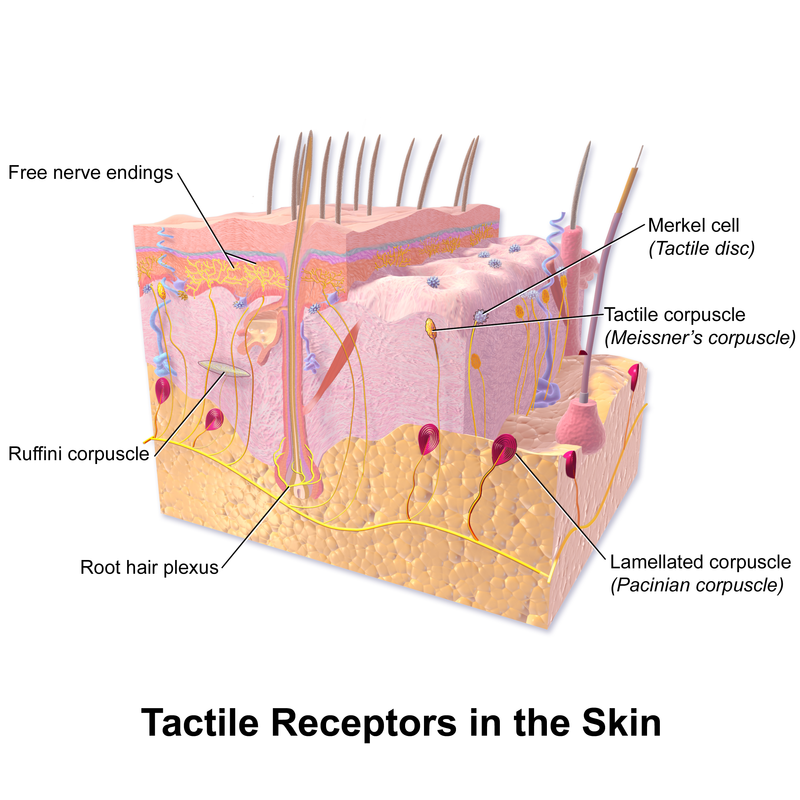
\includegraphics[width=\linewidth]{images/tactileReceptors}
\end{figure}
\end{multicols}
\end{frame}
}

\begin{frame}{La perception tactile}
\begin{table}[]
\centering
\footnotesize
	\begin{tabular}[]{lrrrr}
		\toprule
		\textbf{Nom}			& \textbf{Type}	
		                    & \textbf{Fréquence} & \textbf{Surface de} 
		                    & \textbf{Rôle} \\
		                    & & \textbf{du stimulus} & \textbf{réception} &\\
		\midrule
		Disques de Merkel				& SA-I	& 0-10Hz	& Restreint & Rebord, Pression		\\[0.25em]
		Corp. de Ruffini				& SA-II	& 0-10Hz	& Large & Etirement de la peau	\\[0.25em]
		Corp. de Meissner					& FA-I	& 20-50Hz	& Restreint & Pression	\\[0.25em]
		Corp. de Pacini				& FA-II	& 100-300Hz	& Large & Pression profonde,\\
		& & & & vibration\\
		\bottomrule
	\end{tabular}
	\caption{Caractéristiques des méchanorécepteurs}
\end{table}
\end{frame}

{
\setbeamertemplate{frame footer}{\copyright http://www.ib.cnea.gov.ar}
\begin{frame}{La perception tactile}
\begin{figure}
\centering
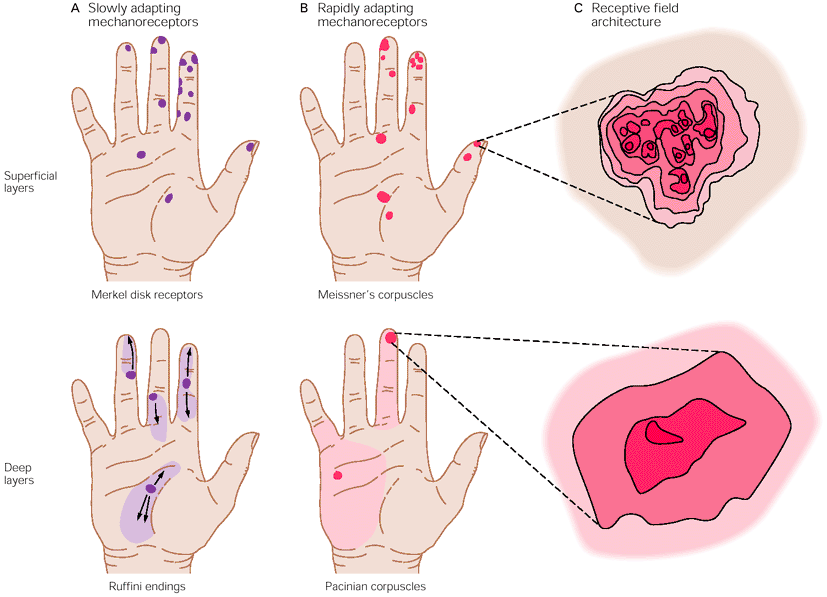
\includegraphics[width=10cm]{images/mechanoreceptors}
\end{figure}
\end{frame}
}
%\note{
%	\begin{itemize}
%		\item Splitshow (Mac OS X)\\\url{https://code.google.com/p/splitshow/}
%		\item pdf-presenter (Windows)\\\url{https://code.google.com/p/pdf-presenter/}
%	\end{itemize} 
%}

{
\setbeamertemplate{frame footer}{\cite{mancini2014whole}}
\begin{frame}{La perception tactile}
\begin{figure}
\centering
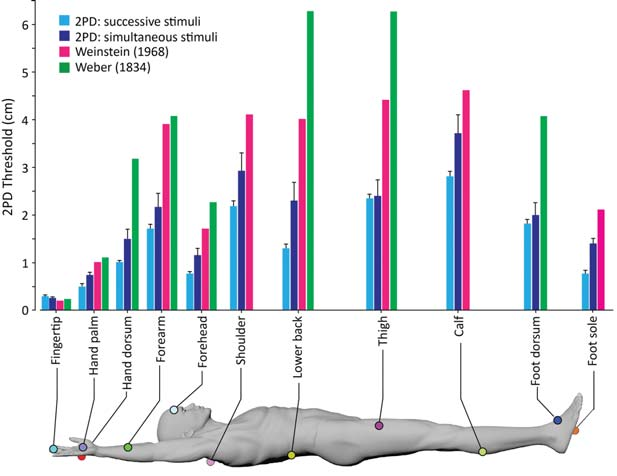
\includegraphics[width=8cm]{images/tactile_acuity}
\end{figure}
\end{frame}
}

{
\setbeamertemplate{frame footer}{\copyright Wikipedia.org}
\begin{frame}{La perception tactile - thermique}
\begin{itemize}
\item Récepteurs thermiques identifiés récemment (Nobel 2021)
\item Les récepteurs mesurent les variations de températures
\begin{itemize}
\item récepteurs au chaud (entre 30 et 46 $^{\circ}C$)
\item récepteurs au froid (entre 10 et 35 $^{\circ}C$)
\end{itemize}
\end{itemize}
\begin{figure}
\centering
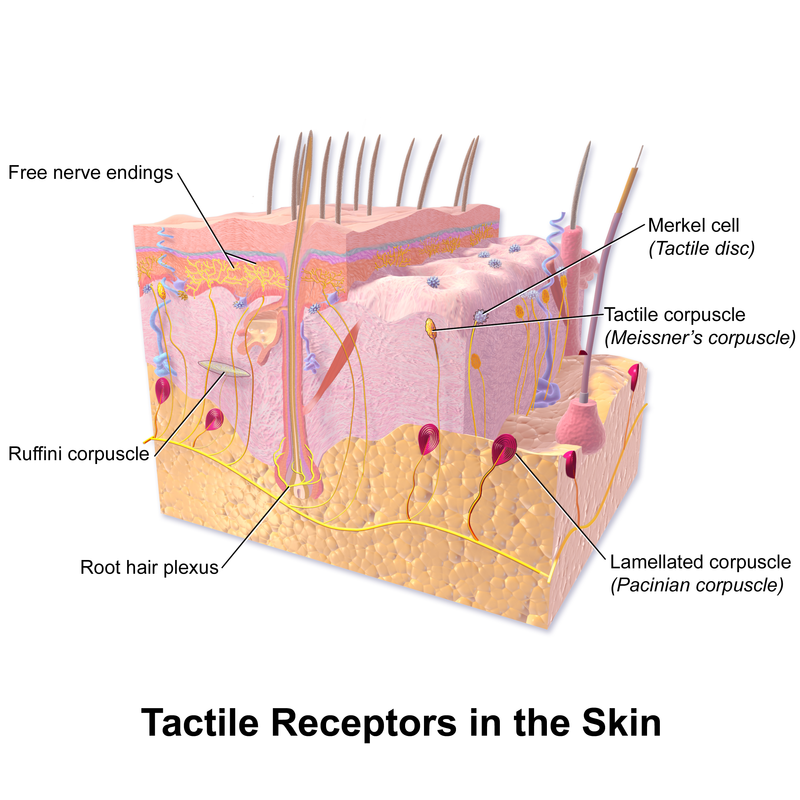
\includegraphics[width=4cm]{images/tactileReceptors}
\end{figure}
\end{frame}
}

\subsection{Illusions tactiles}
{
\setbeamertemplate{frame footer}{\cite{Hayward2008b}}
\begin{frame}{Illusions tactiles}
\begin{figure}
\centering
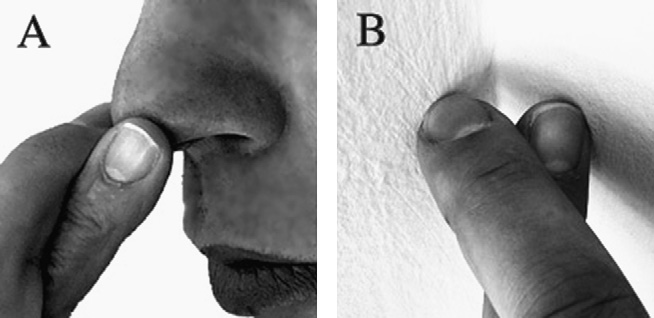
\includegraphics[width=8cm]{images/illusions_aristote}
\caption{Illusion d'Aristote. Lorsque les doigts sont croisés, deux surfaces sont perçues au lieu d'une (A). L'illusion inverse consiste à ne ressentir qu'une surface au lieu de deux (B).}
\end{figure}
\end{frame}

\begin{frame}{Illusions tactiles}
\begin{figure}
\centering
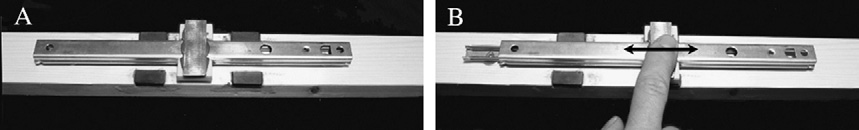
\includegraphics[width=\linewidth]{images/illusions_bump}
\caption{Illusion de bosses et creux. Réalisée avec une glissière et des aimants. Les aimants vont réduire la vitesse de déplacement de la glissière, induisant une illusion de bosses et de creux.}
\end{figure}
\end{frame}
}

{
\setbeamertemplate{frame footer}{\cite{Tan1997c}}
\begin{frame}{Illusions tactiles}
\begin{figure}
\centering
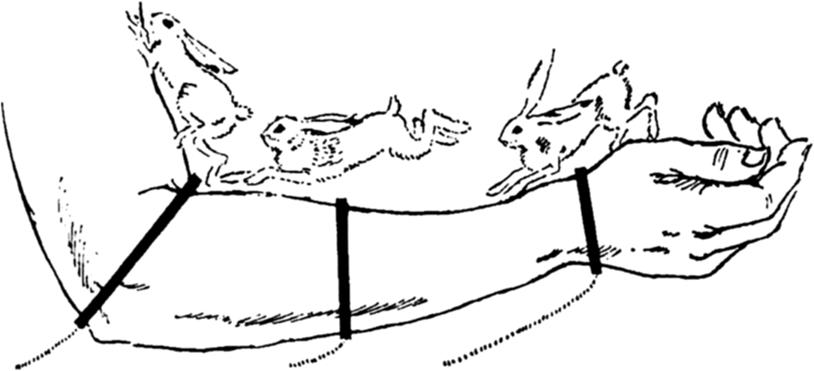
\includegraphics[width=10cm]{images/illusions_rabbit}
\caption{"Cutaneous rabbit illusion". Lorsque 3 vibrations sont appliquées successivement sur la surface de la peau, seul un stimulus continu est ressenti.}
\end{figure}
\end{frame}
}

{
\setbeamertemplate{frame footer}{\cite{Salzer2007}}
\begin{frame}{Illusions tactiles}
\begin{figure}
\centering
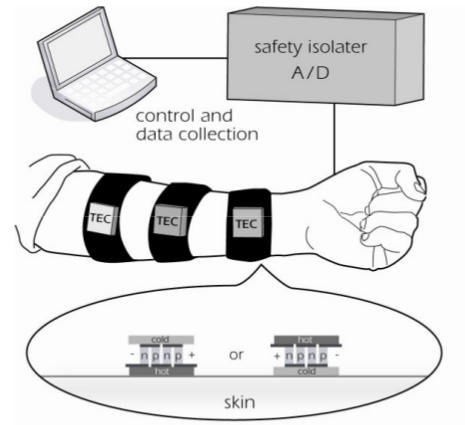
\includegraphics[width=5cm]{images/thermalgrill}
\caption{Illusion du grill. Stimuli chauds (40$^{\circ}C$) et froids (20$^{\circ}C$) appliqués successivement sur la peau. Une sensation de brûlure apparait.}
\end{figure}
\end{frame}
}

\subsection{Interfaces Tactile}
\begin{frame}{Interfaces tactiles - Contact}
\begin{itemize}
\item Vibreurs
\item Solénoïdes
\end{itemize}

\begin{multicols}{2}
\begin{figure}
\centering
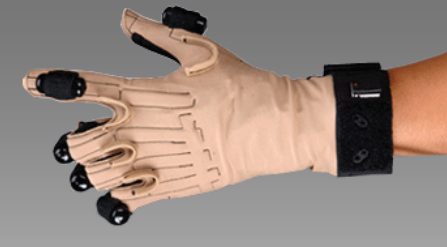
\includegraphics[width=3cm]{images/cybertouch}
\caption{\copyright Cybertouch.com}
\end{figure}
%\movie[externalviewer]{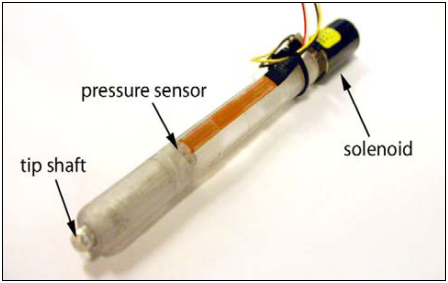
\includegraphics[width=4cm]{images/hapticPen.PNG}}{videos/Haptic_Pen.mp4}
%\includemovie[poster,text={\small(Loading Circle-m-increase3.mp4)}]{4cm}{4cm}{videos/Haptic_Pen.mp4}
\begin{figure}
\centering
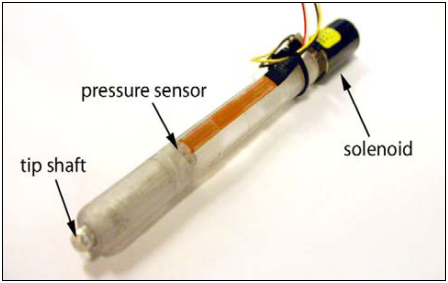
\includegraphics[width=3cm]{images/hapticPen}
\vspace{-0.2cm}
\caption{\cite{Lee2004}}
\end{figure}
\end{multicols}

\vspace{-1cm}

\begin{figure}
\centering
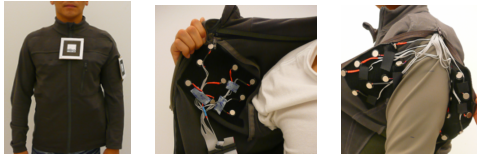
\includegraphics[width=8cm]{images/Rahman2010}
\caption{\cite{Rahman2010}}
\end{figure}

\end{frame}


{
\setbeamertemplate{frame footer}{\copyright precisionmicrodrives.com}
\begin{frame}{Moteur à masse excentrique (ERM)}
\begin{figure}
\centering
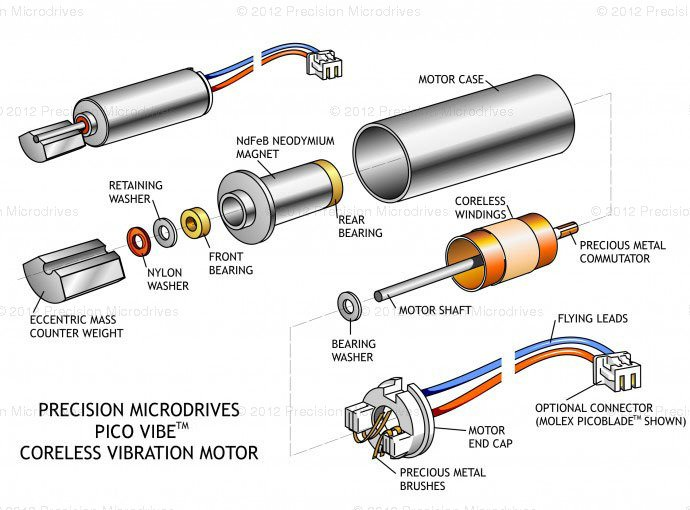
\includegraphics[width=\linewidth]{images/ERM}
\end{figure}
\end{frame}

\begin{frame}{Moteur à masse excentrique (ERM)}
\begin{figure}
\centering
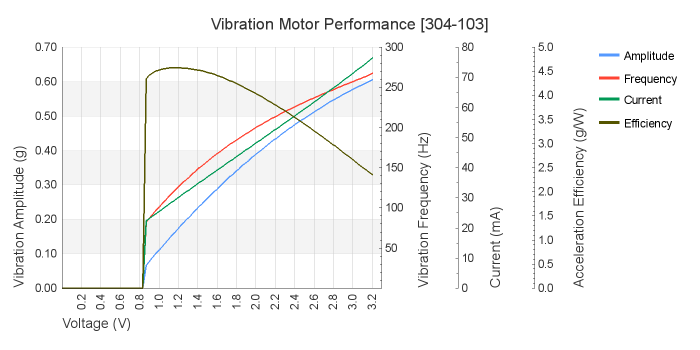
\includegraphics[width=\linewidth]{images/ERM_output}
\end{figure}
\end{frame}
}

\begin{frame}{Exemple: manette Xbox One}
\begin{figure}
\centering
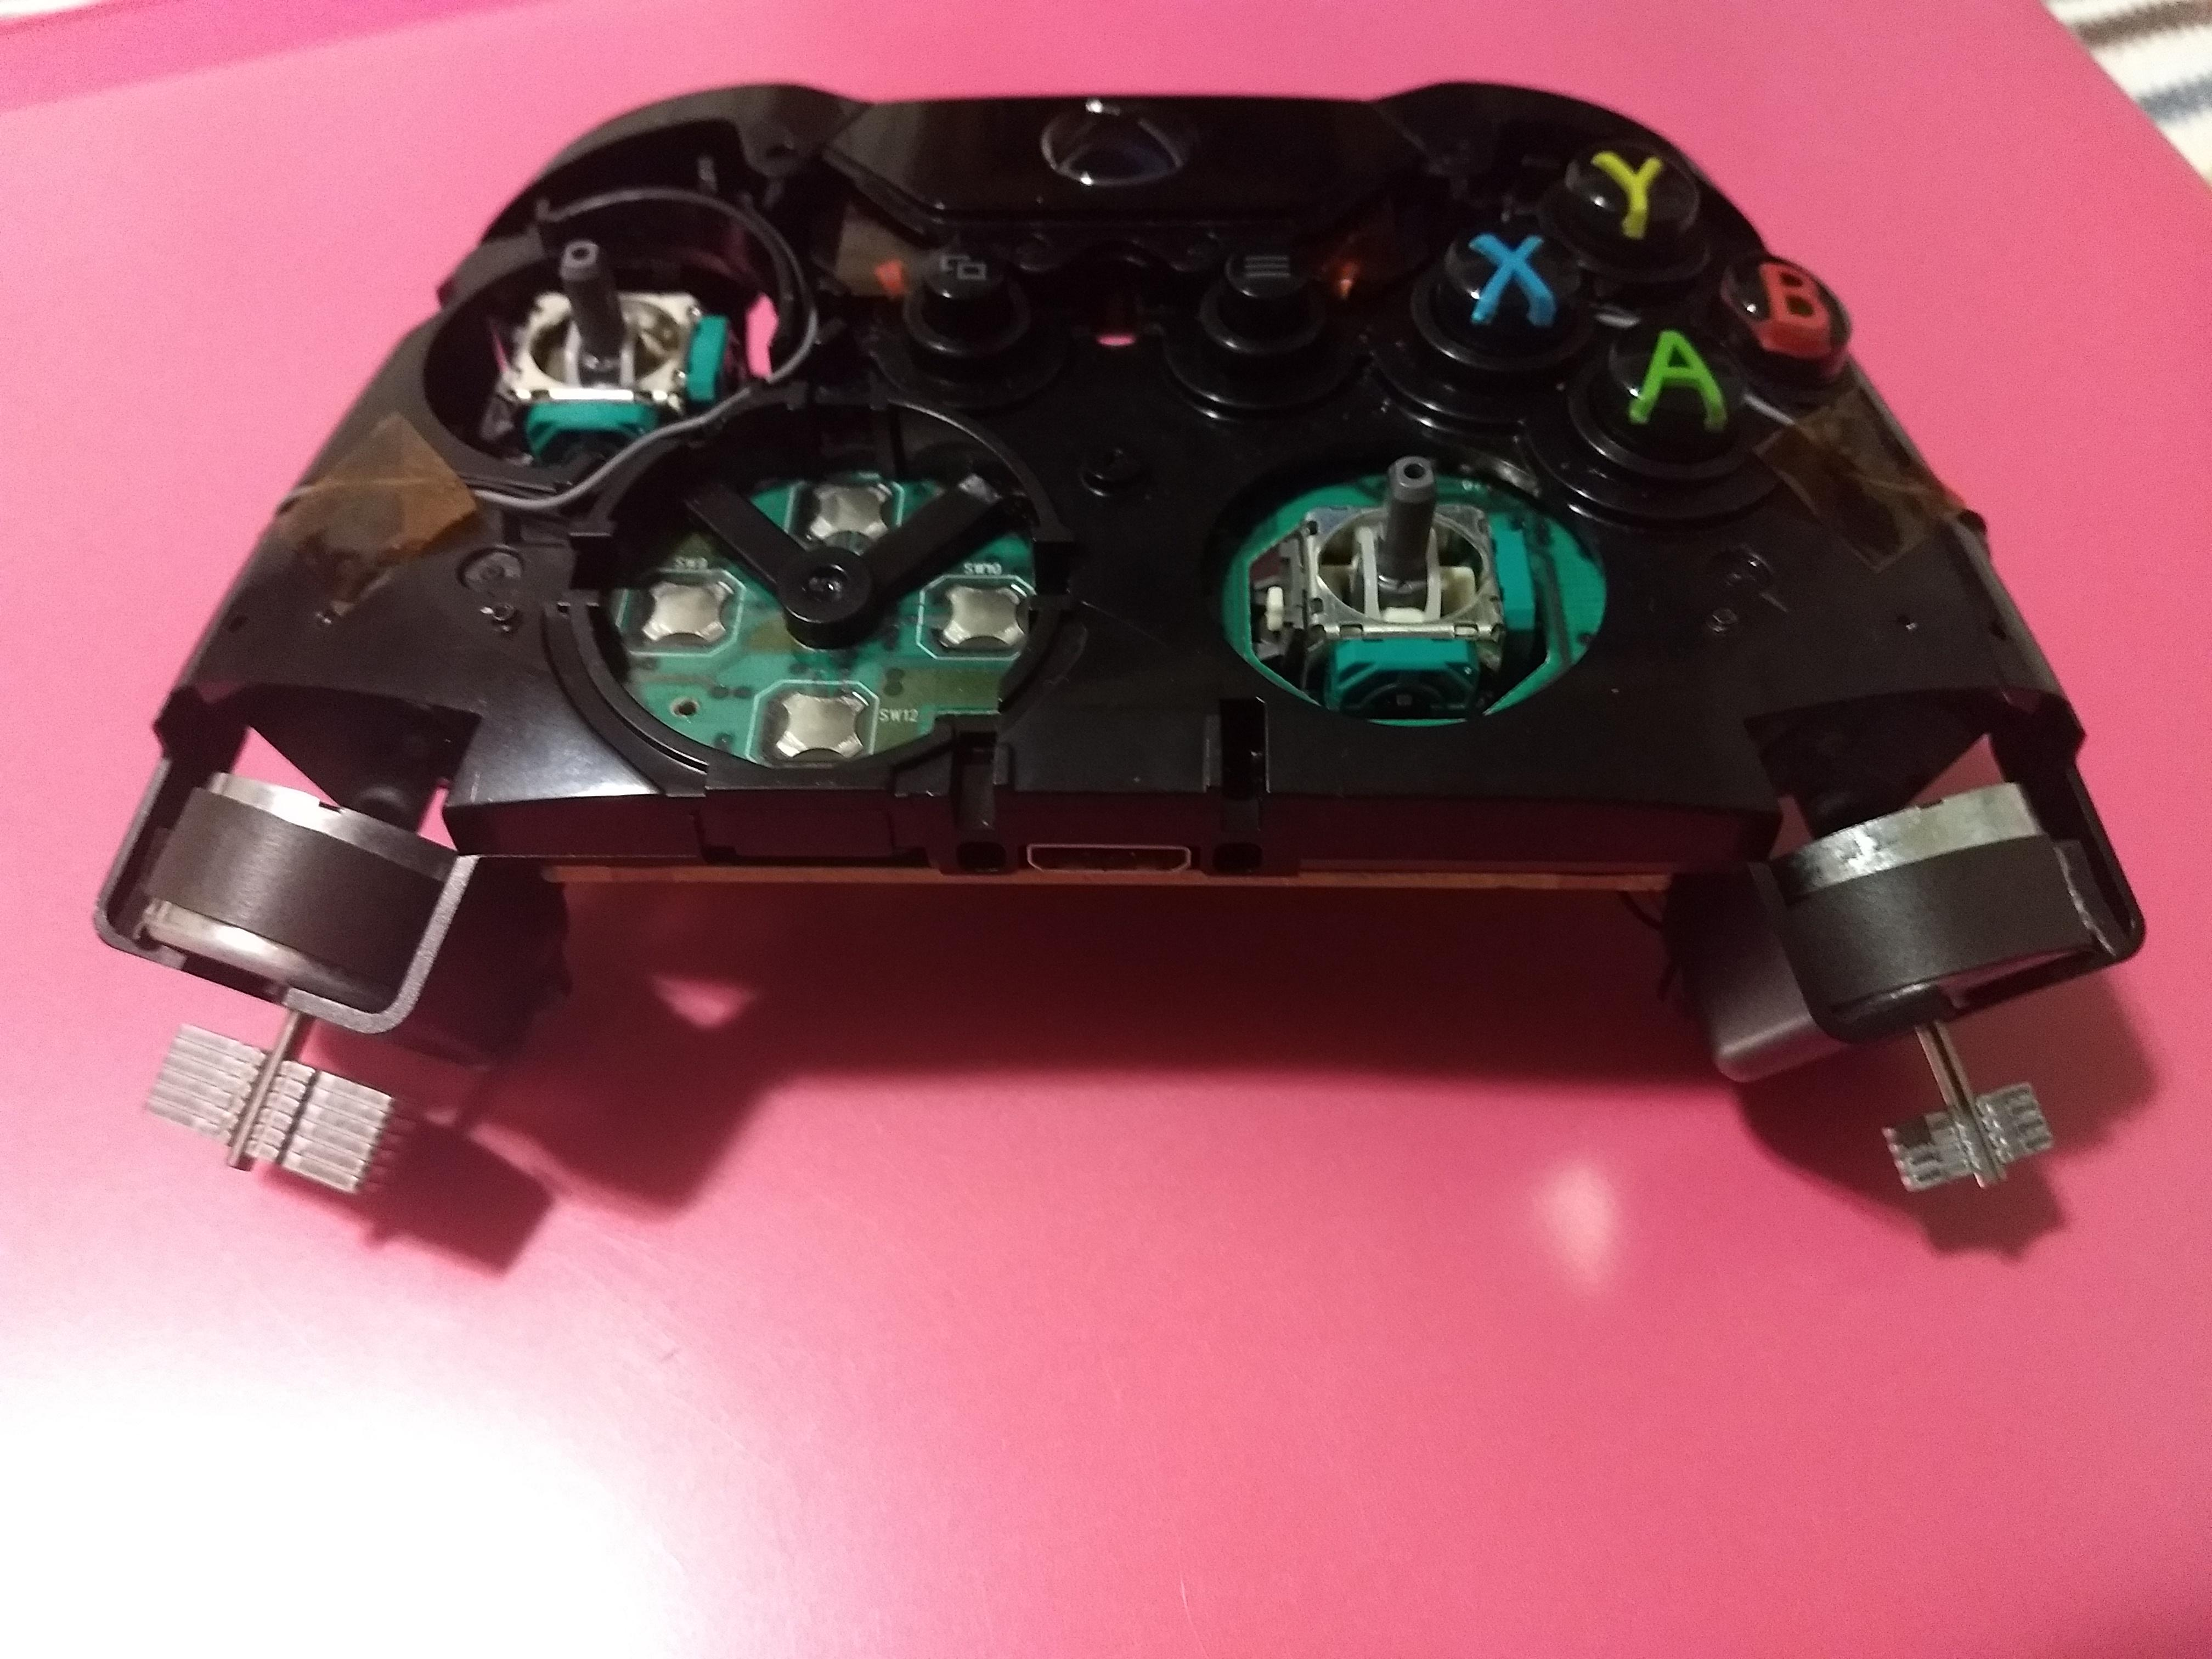
\includegraphics[width=\linewidth]{images/xboxone}
\end{figure}
\end{frame}

{
\setbeamertemplate{frame footer}{\copyright precisionmicrodrives.com}
\begin{frame}{Moteur linéaire (LRA)}
\begin{figure}
\centering
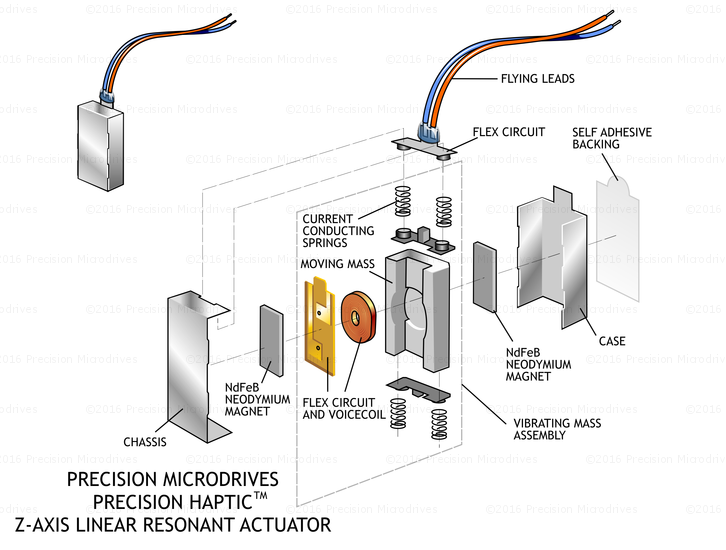
\includegraphics[width=\linewidth]{images/lra}
\end{figure}
\end{frame}

\begin{frame}{Moteur linéaire (LRA)}
\begin{figure}
\centering
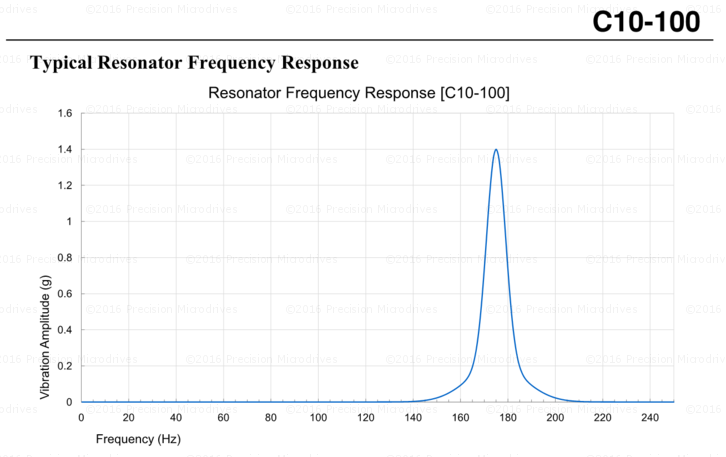
\includegraphics[width=\linewidth]{images/LRA_output}
\end{figure}
\end{frame}
}

{
\setbeamertemplate{frame footer}{\copyright ifixit.com}
\begin{frame}{Exemple: manette Switch}
\begin{figure}
\centering
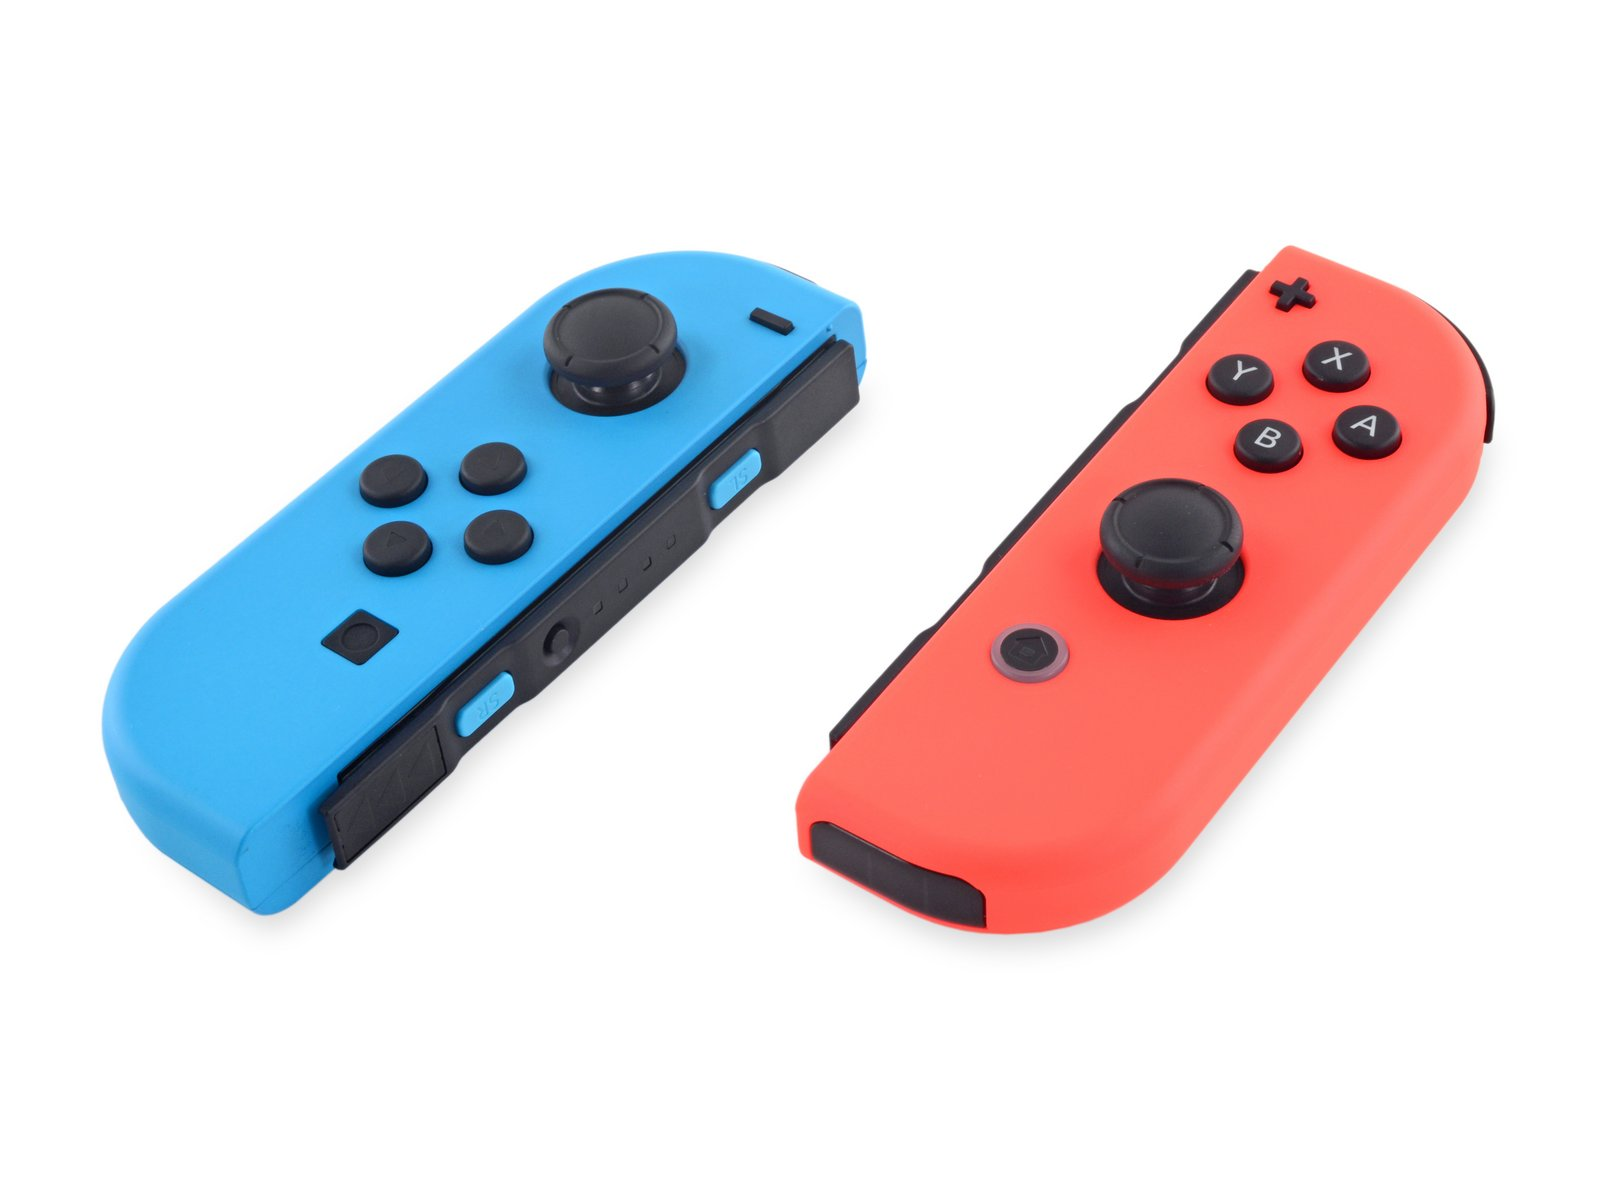
\includegraphics[width=0.4\linewidth]{images/switch1}
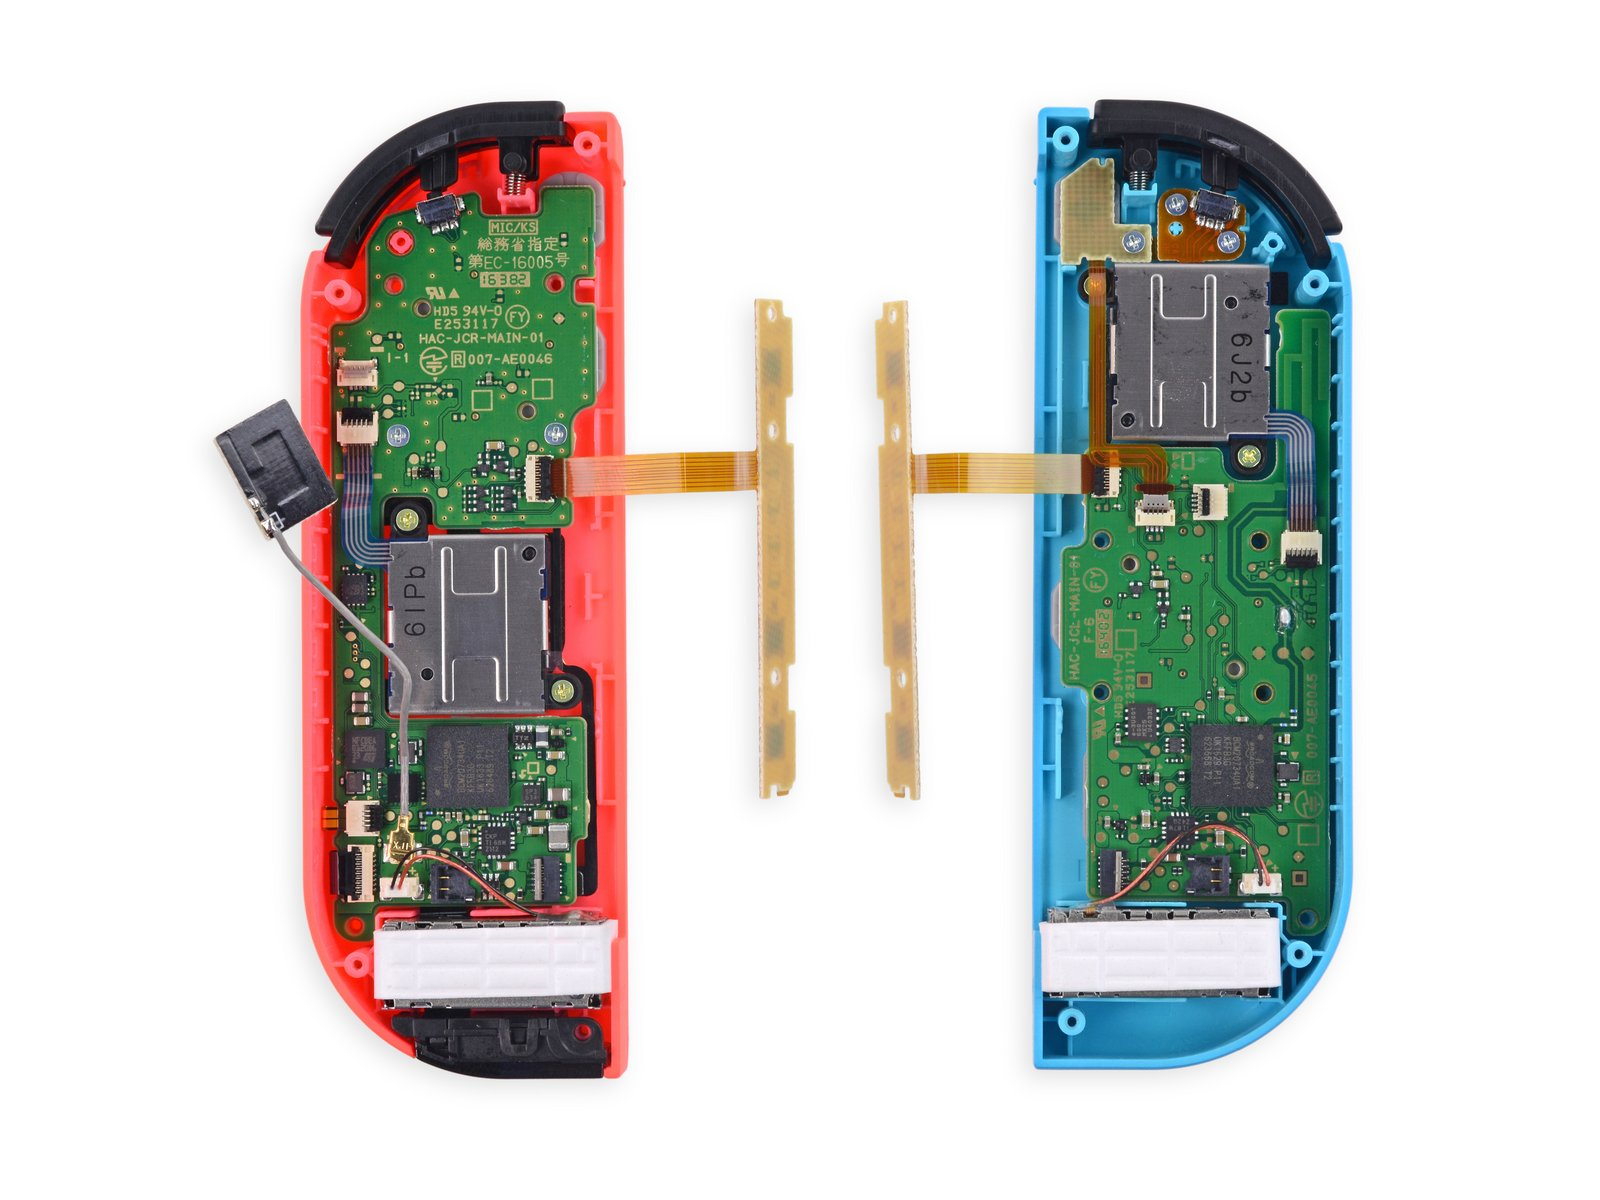
\includegraphics[width=0.4\linewidth]{images/switch2}
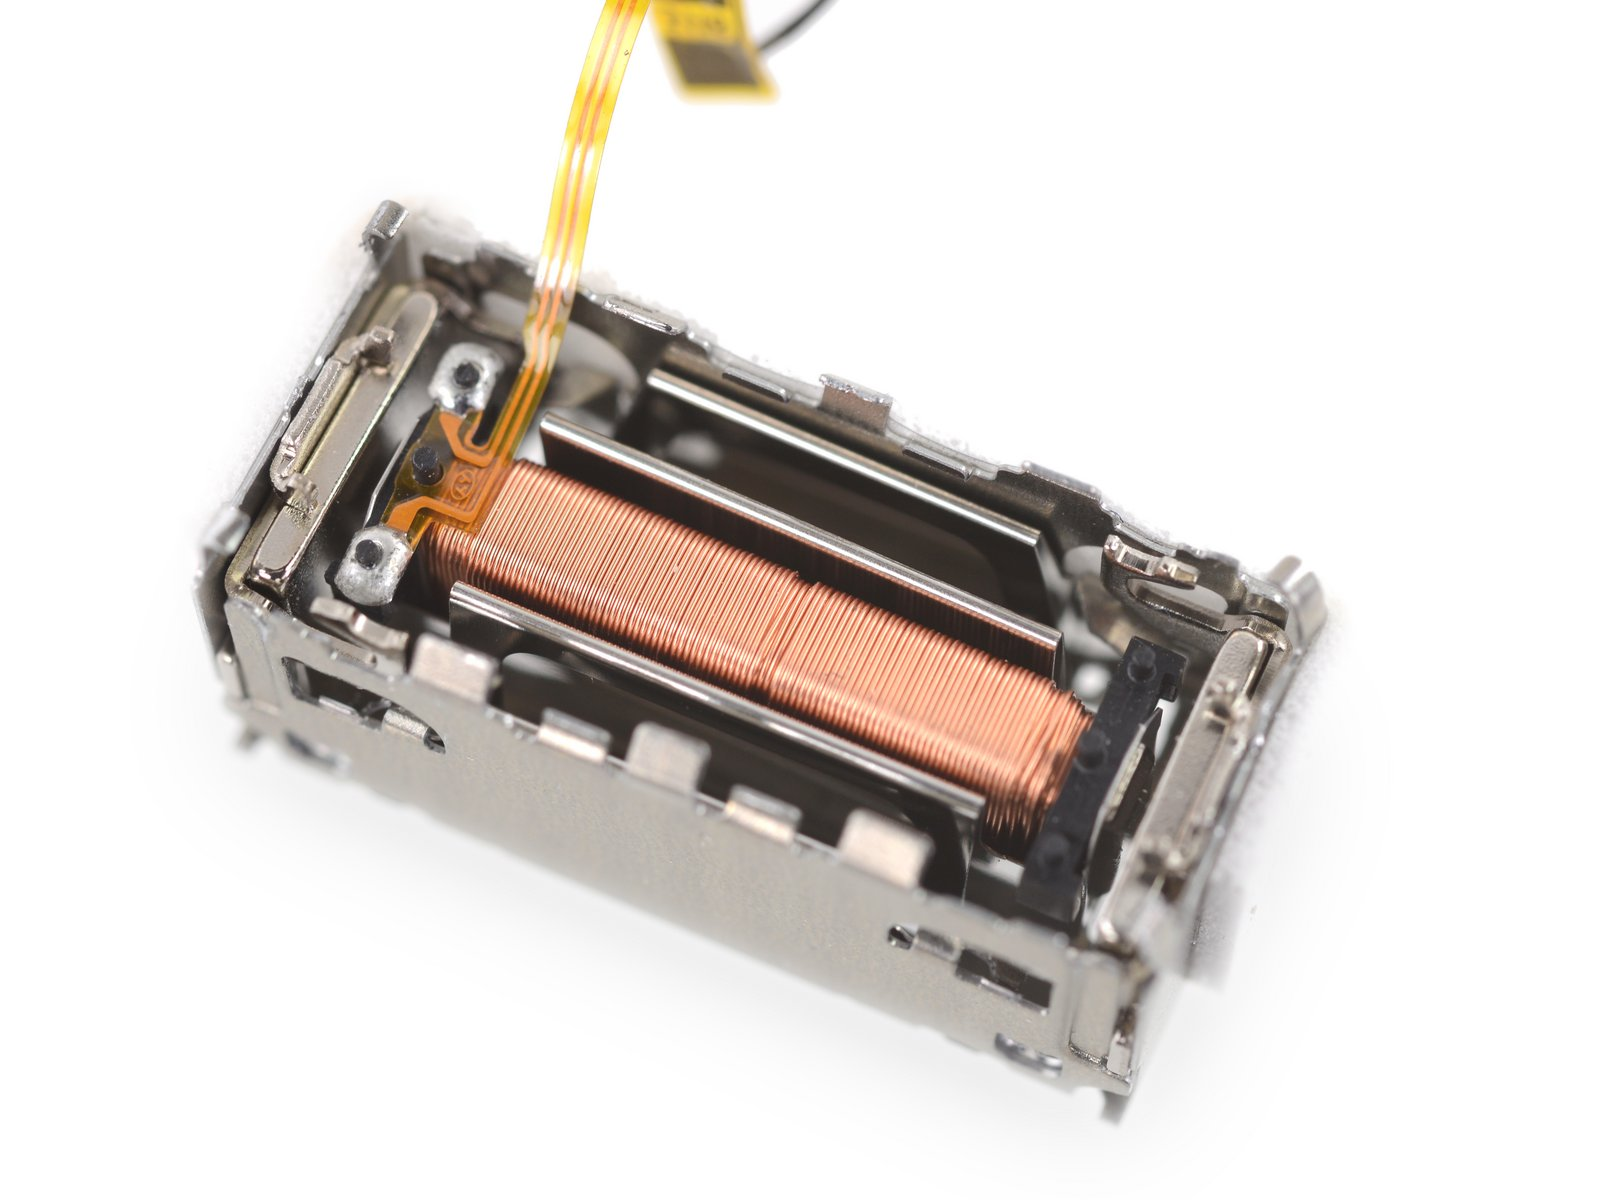
\includegraphics[width=0.4\linewidth]{images/HDRumble1}
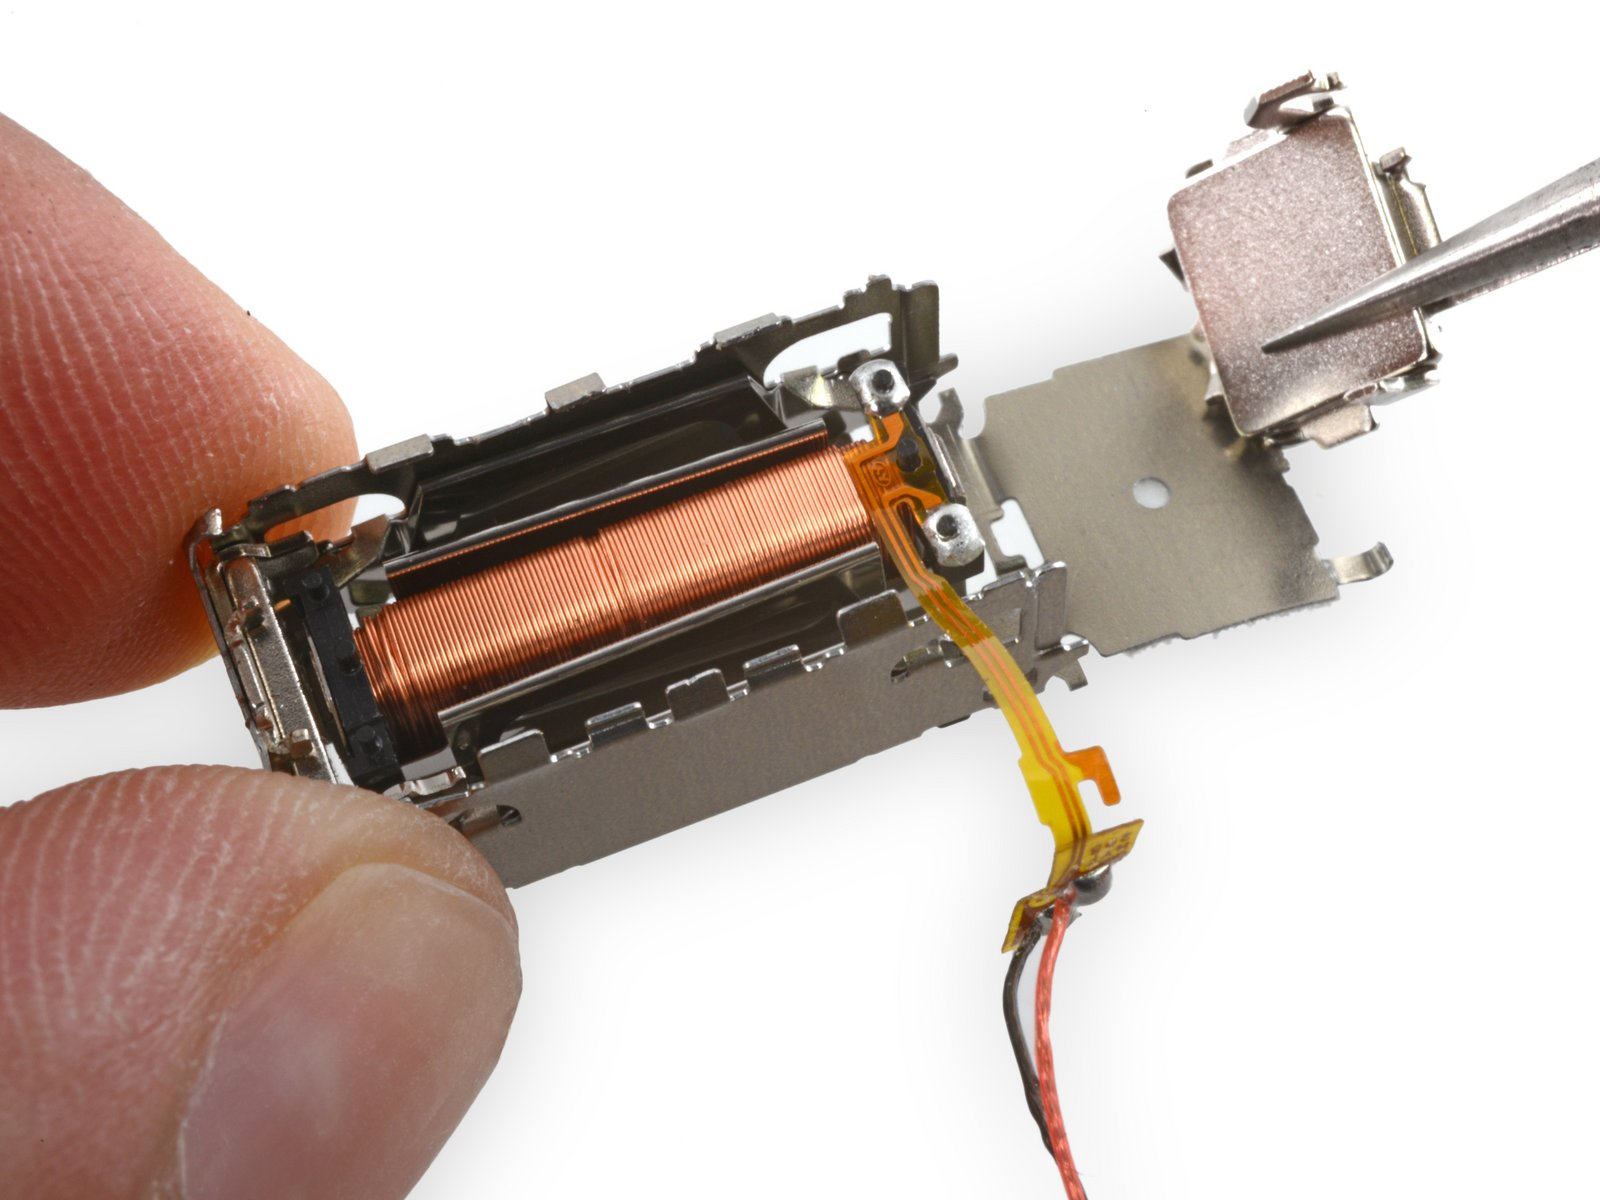
\includegraphics[width=0.4\linewidth]{images/HDRumble2}
\end{figure}
\end{frame}
}

{
\setbeamertemplate{frame footer}{\copyright actronika.com}
\begin{frame}{Voice-coil}
\begin{figure}
\centering
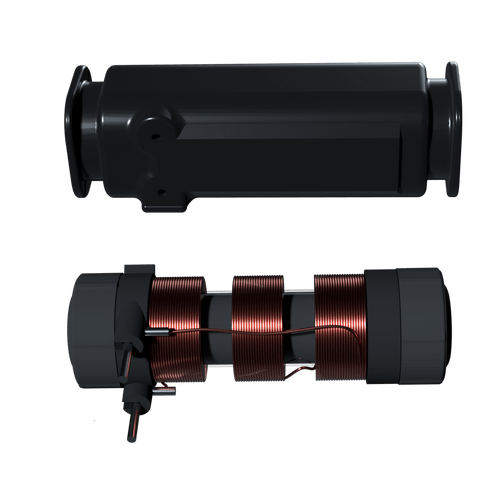
\includegraphics[width=0.45\linewidth]{images/voice-coil_2}
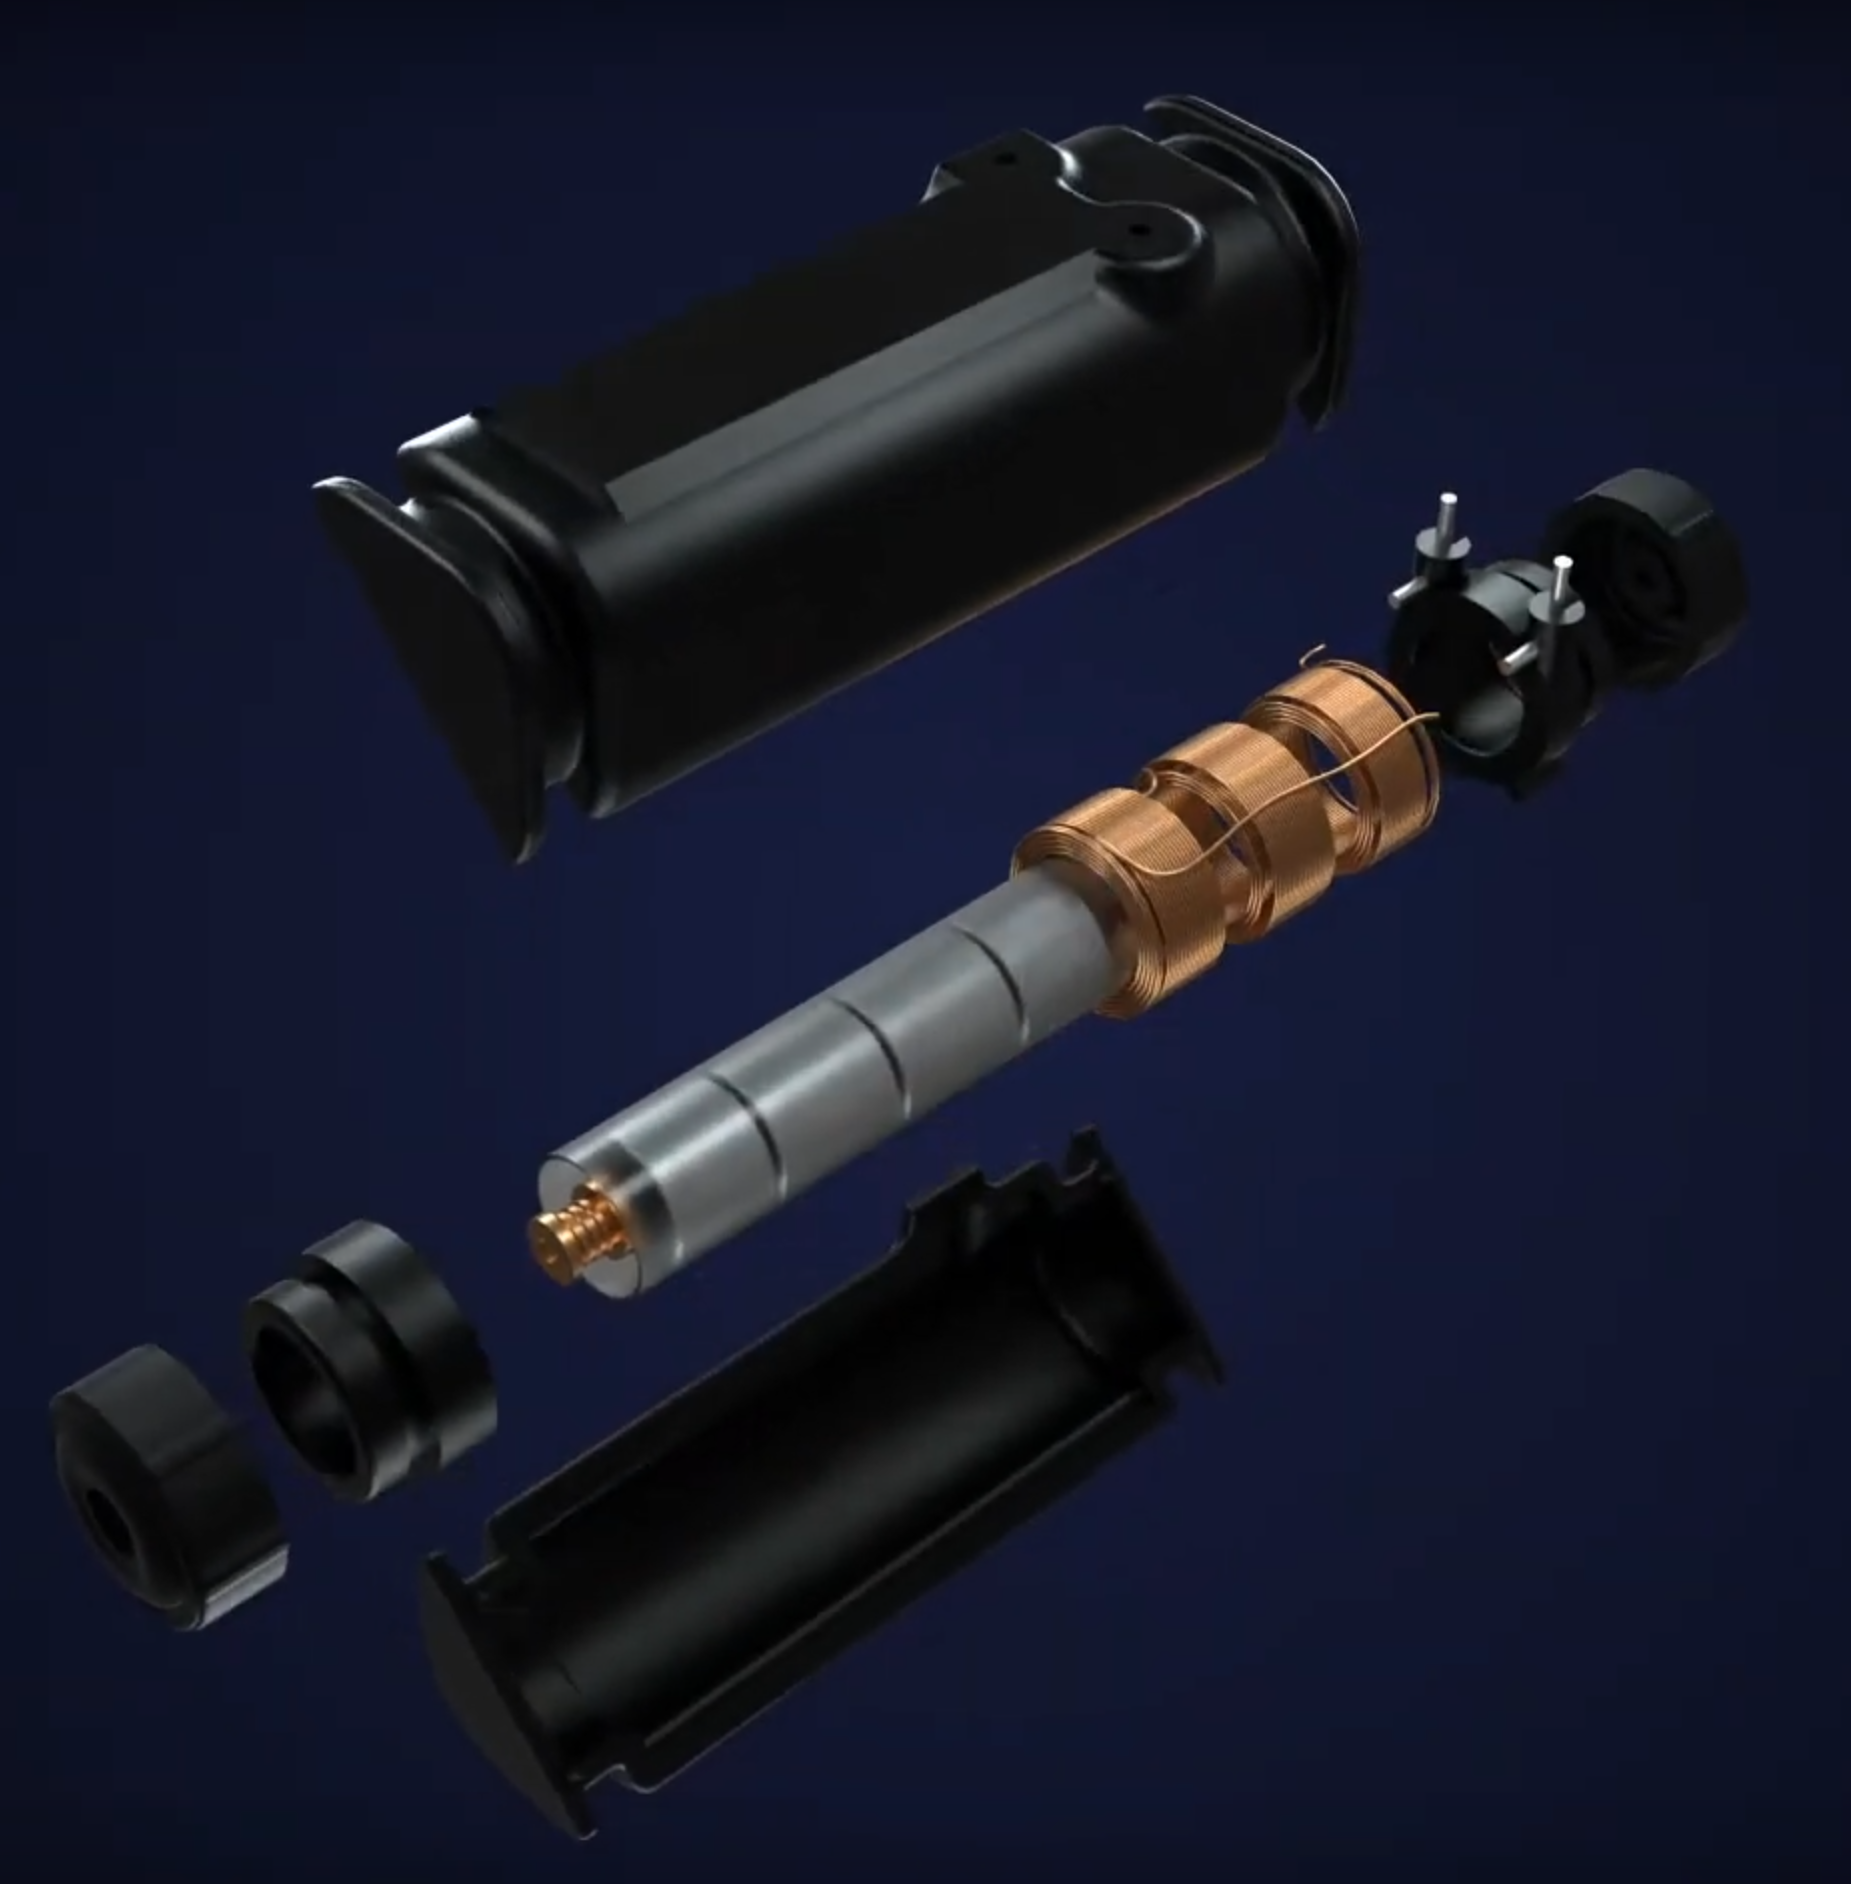
\includegraphics[width=0.45\linewidth]{images/voice-coil}
\end{figure}
\end{frame}
}

{
\setbeamertemplate{frame footer}{\copyright actronika.com}
\begin{frame}{Voice-coil}
\begin{figure}
\centering
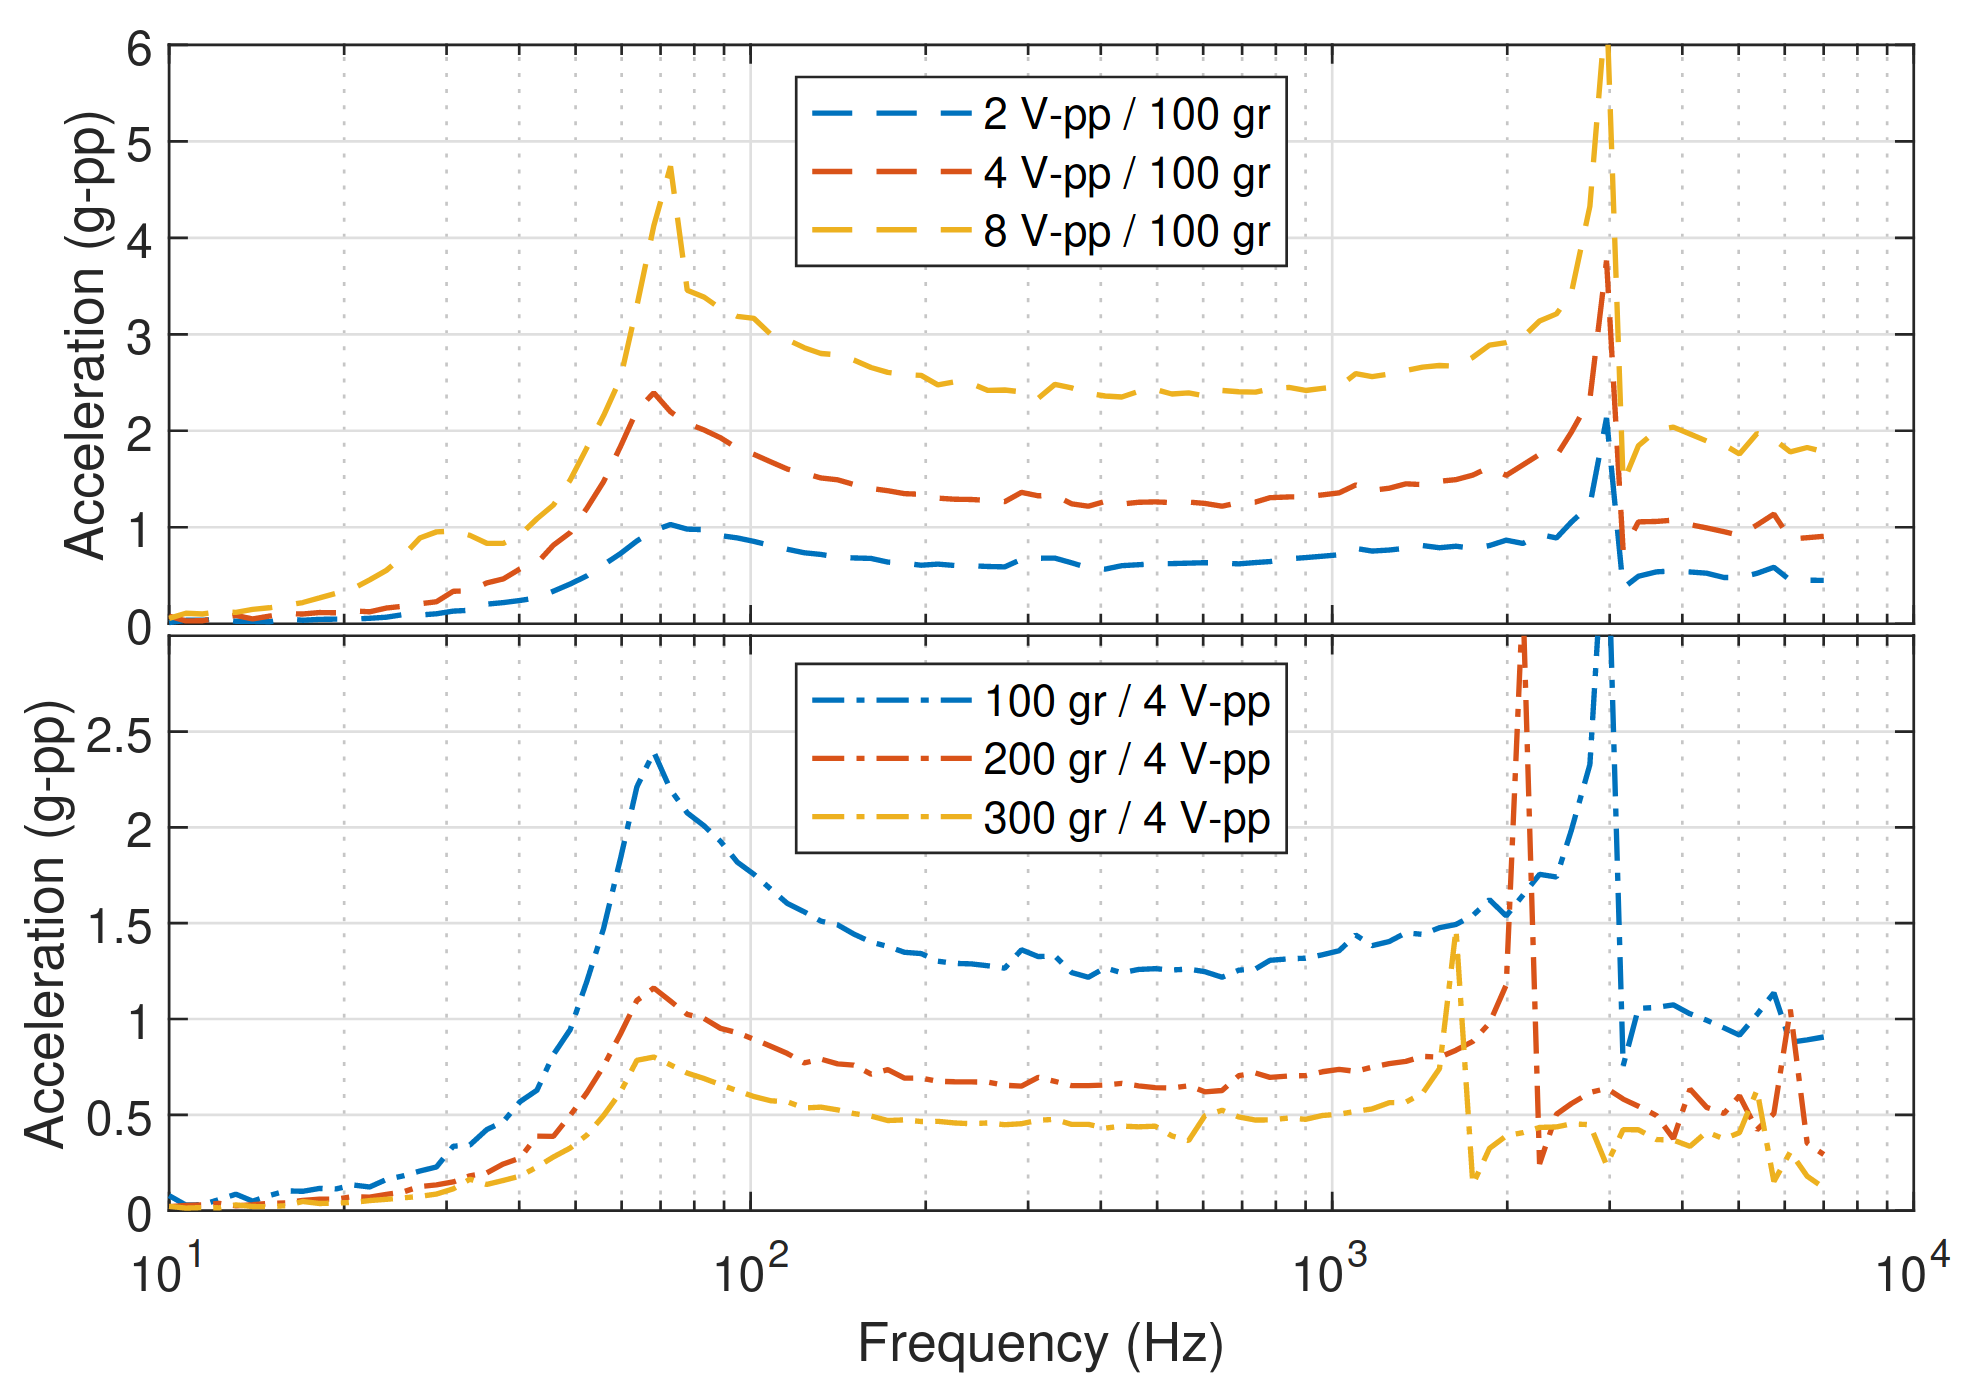
\includegraphics[width=\linewidth]{images/voice-coil_bandwidth}
\end{figure}
\end{frame}
}


{
\setbeamertemplate{frame footer}{\cite{choi2020development}}
\begin{frame}{Interfaces tactiles - Contact}
\begin{figure}
\centering
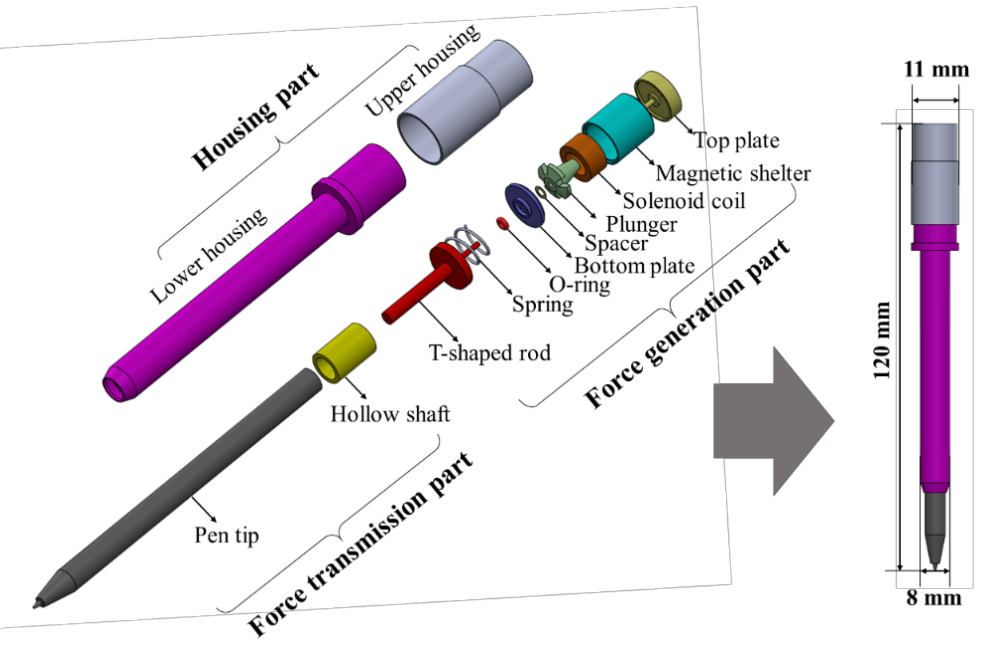
\includegraphics[width=\linewidth]{images/stylus}
\end{figure}
\end{frame}
}

{
\setbeamertemplate{frame footer}{\cite{benko2016}}
\begin{frame}{Interfaces tactiles - Contact}
\begin{figure}
\href{run:videos/microsoft_texture.mp4}{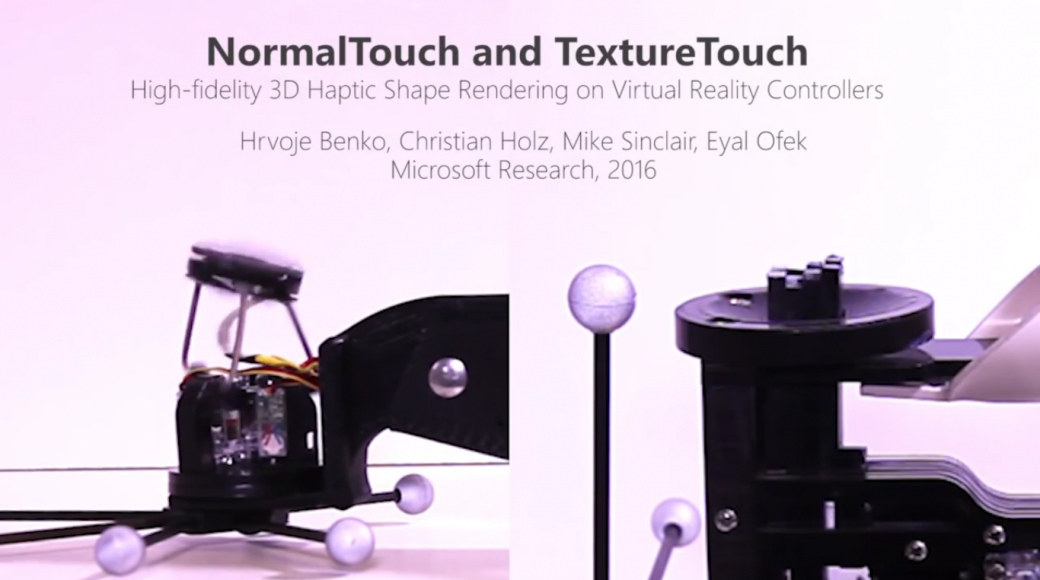
\includegraphics[width=\linewidth]{images/microsoft_textureTouch}}
\end{figure}

\end{frame}
}

{
\setbeamertemplate{frame footer}{\copyright ifixit.com}
\begin{frame}{Exemple: manette PS5}
\begin{figure}
\centering
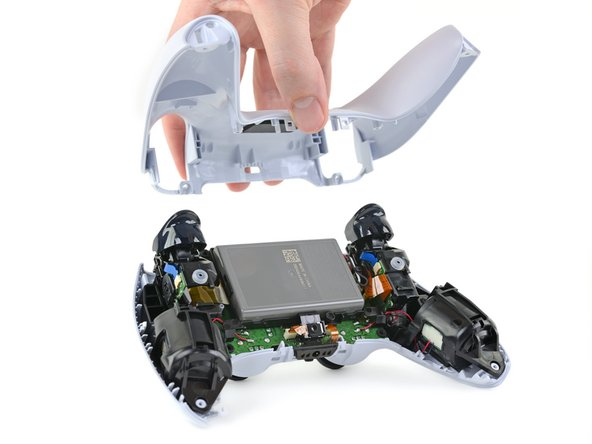
\includegraphics[width=0.4\linewidth]{images/ps5_open}
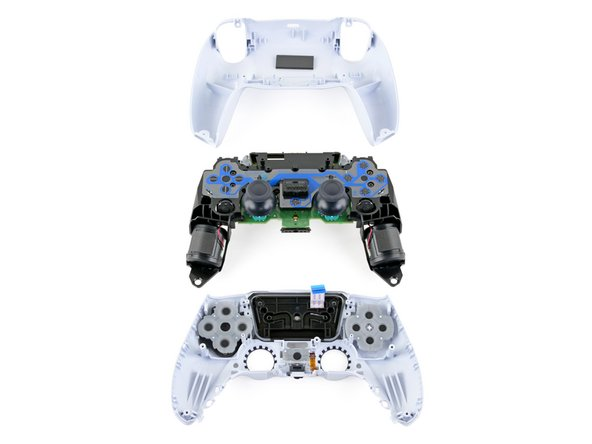
\includegraphics[width=0.4\linewidth]{images/ps5_breakdown}
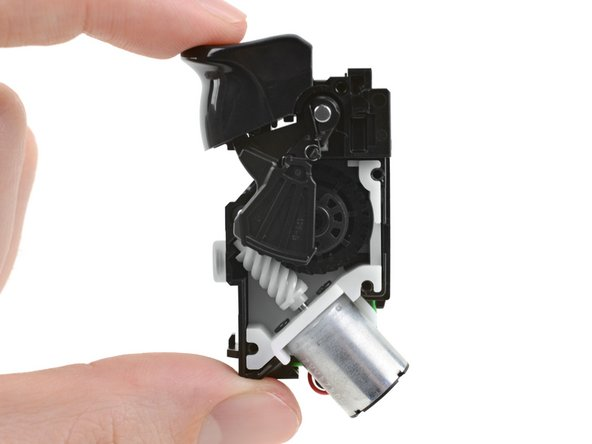
\includegraphics[width=0.4\linewidth]{images/ps5_trigger}
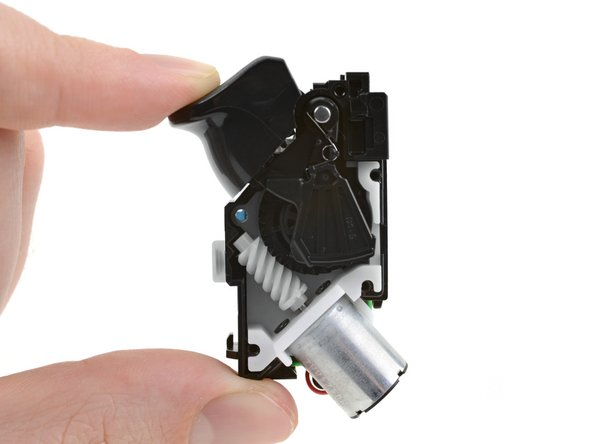
\includegraphics[width=0.4\linewidth]{images/ps5_trigger2}
\end{figure}
\end{frame}
}

\begin{frame}{Interfaces tactiles - Texture}
\begin{multicols}{2}

\begin{itemize}
\item Matrice de picots
\item Actuateur piezo-electrique
\item Vibration electrostatique
\end{itemize}

\begin{figure}
\centering
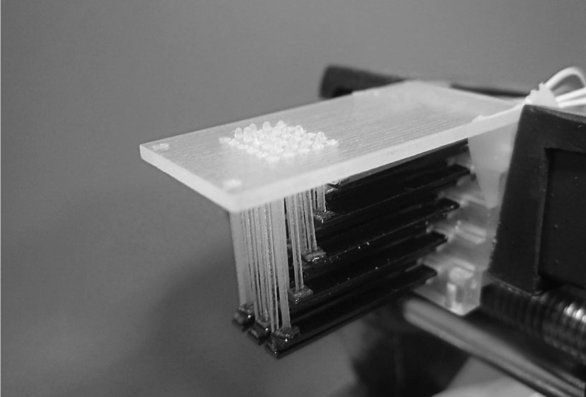
\includegraphics[width=4cm]{images/texture}
\caption{\cite{Yang2008}}
\end{figure}

\begin{figure}
\centering
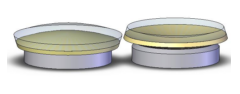
\includegraphics[width=4cm]{images/piezo}
\end{figure}

%\vspace{-1cm}
\begin{figure}
\centering
%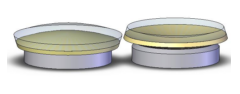
\includegraphics[width=4cm]{images/piezo}
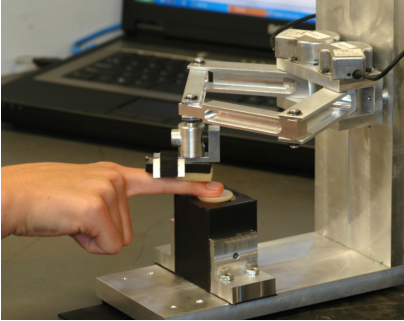
\includegraphics[width=4cm]{images/piezo2}
\caption{\cite{Winfield2007}}
\end{figure}

\end{multicols}

%\vspace{-0.5cm}
%\begin{figure}
%\centering
%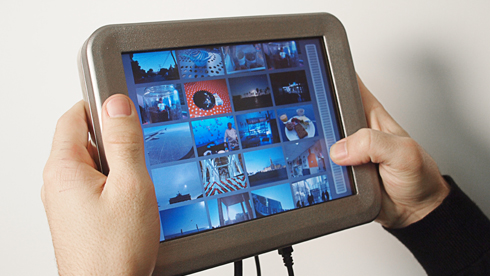
\includegraphics[width=4cm]{images/teslatouch-03}
%\caption{\cite{bau2010}}
%\end{figure}

%\begin{figure}
%\centering
%\movie[externalviewer]{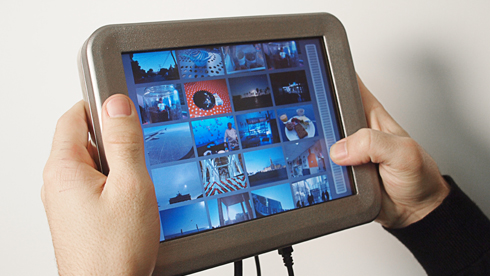
\includegraphics[width=4cm]{images/teslatouch-03}}{videos/TeslaTouch.mov}
%\linebreak
%
\includegraphics[width=\linewidth]{images/none}{\copyright \mbox{Bau et al., 2010}}
%\end{figure}


\end{frame}

{
\setbeamertemplate{frame footer}{\cite{bau2010}}
\begin{frame}{Interfaces tactiles - Texture}
\begin{figure}
\href{run:videos/TeslaTouch.mov}{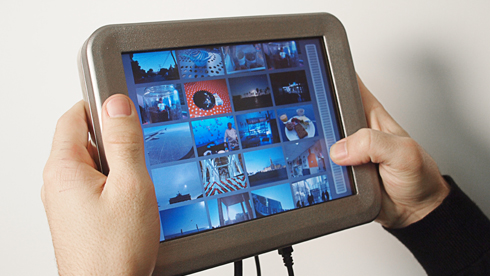
\includegraphics[width=\linewidth]{images/teslatouch-03}}
\end{figure}
\end{frame}
}

\begin{frame}{Interfaces tactiles - pression sans contact}
\begin{multicols}{2}

\begin{itemize}
\item Ultrasonic transmitters array
\item Projecteur de flux d'air
\end{itemize}

\begin{figure}
\centering
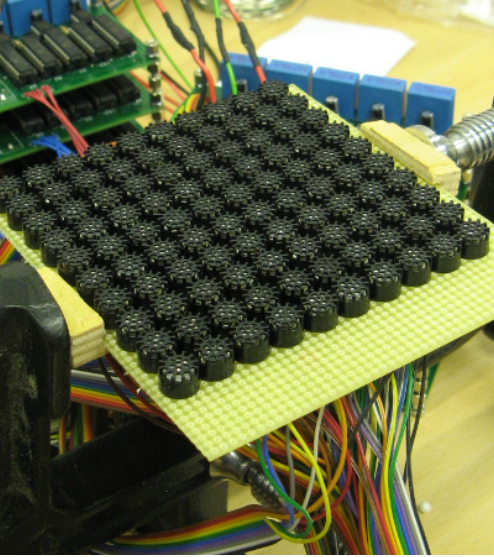
\includegraphics[width=2.25cm]{images/ultrahaptics}
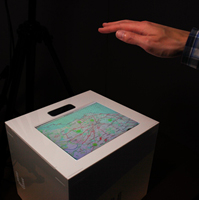
\includegraphics[width=2.5cm]{images/ultrahaptics_project_photo}
\caption{\cite{Alexander2011}}
\end{figure}

%\begin{figure}
%\centering
%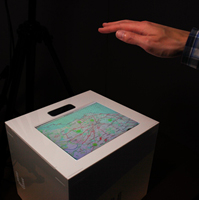
\includegraphics[width=2cm]{images/ultrahaptics_project_photo}
%\end{figure}

\begin{figure}
\centering
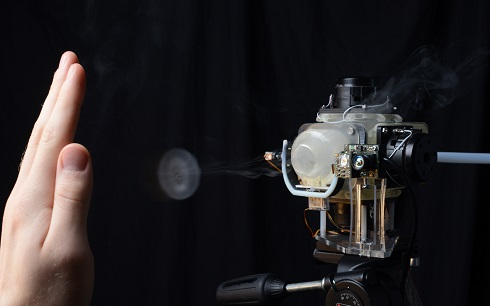
\includegraphics[width=4cm]{images/AIREALVortexRingFig}
%\caption{\cite{Sodhi2013}}
%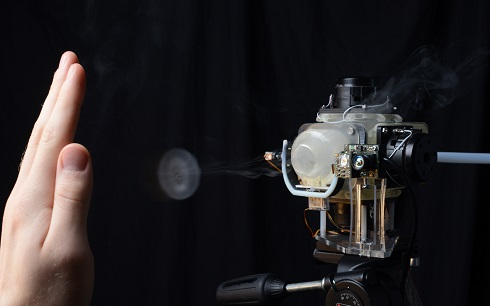
\includegraphics[width=4cm]{images/AIREALVortexRingFig}{}
\end{figure}
\vspace{-1.5cm}
\begin{figure}
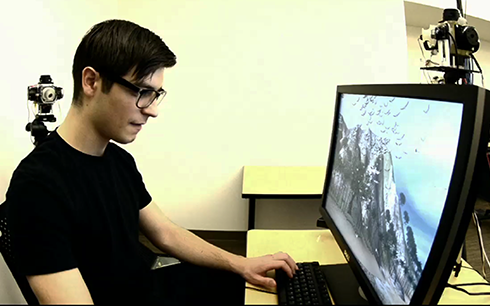
\includegraphics[width=4cm]{images/aireal2}
\caption{\cite{Sodhi2013}}
\end{figure}

\end{multicols}
\end{frame}

{
\setbeamertemplate{frame footer}{\cite{Sodhi2013}}
\begin{frame}{Interfaces tactiles - Pression sans contact}
\begin{figure}
\href{run:videos/Aireal.mp4}{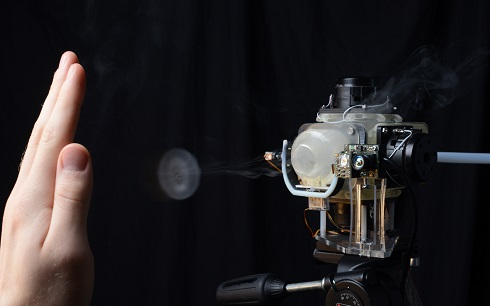
\includegraphics[width=\linewidth]{images/AIREALVortexRingFig}}
\end{figure}
\end{frame}
}

\begin{frame}{Interfaces tactiles - thermique}
\begin{multicols}{2}

\begin{itemize}
\item Ventilateur + source de chaleur
\item Module Peltier
\end{itemize}

\begin{figure}
\centering
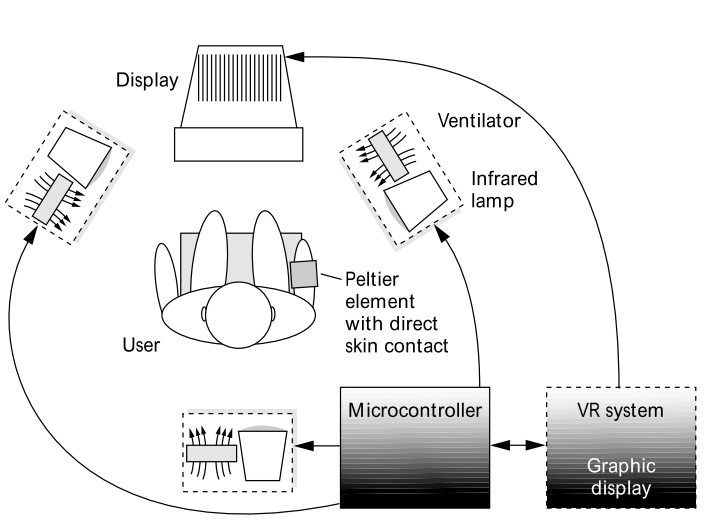
\includegraphics[width=\linewidth]{images/thermalFeedback}\caption{\cite{Dionisio1997}}
\end{figure}

\begin{figure}
\centering
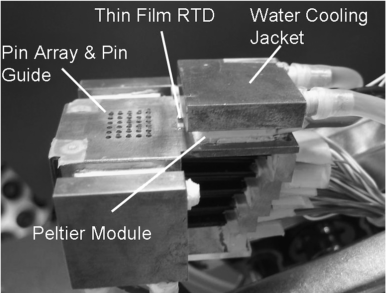
\includegraphics[width=4cm]{images/peltier}
\end{figure}

\begin{figure}
\centering
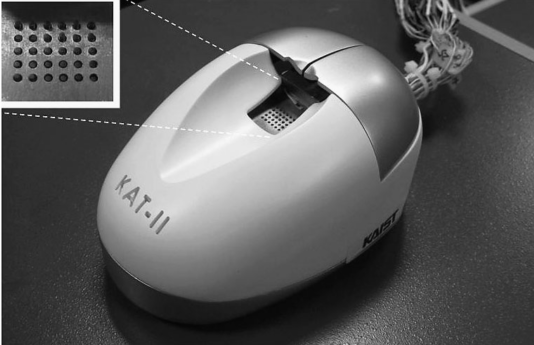
\includegraphics[width=4cm]{images/katII}
\caption{\cite{Yang2008}}
\end{figure}

\end{multicols}
\end{frame}

{
\setbeamertemplate{frame footer}{\copyright Wikipedia.org}
\begin{frame}{Effet Peltier}
\begin{itemize}
\item Le passage du courant dans les semi-conducteurs N et P provoquent un flux thermique
\item Découvert en 1834 par Jean-Charles Peltier
\end{itemize}
\begin{figure}
\centering
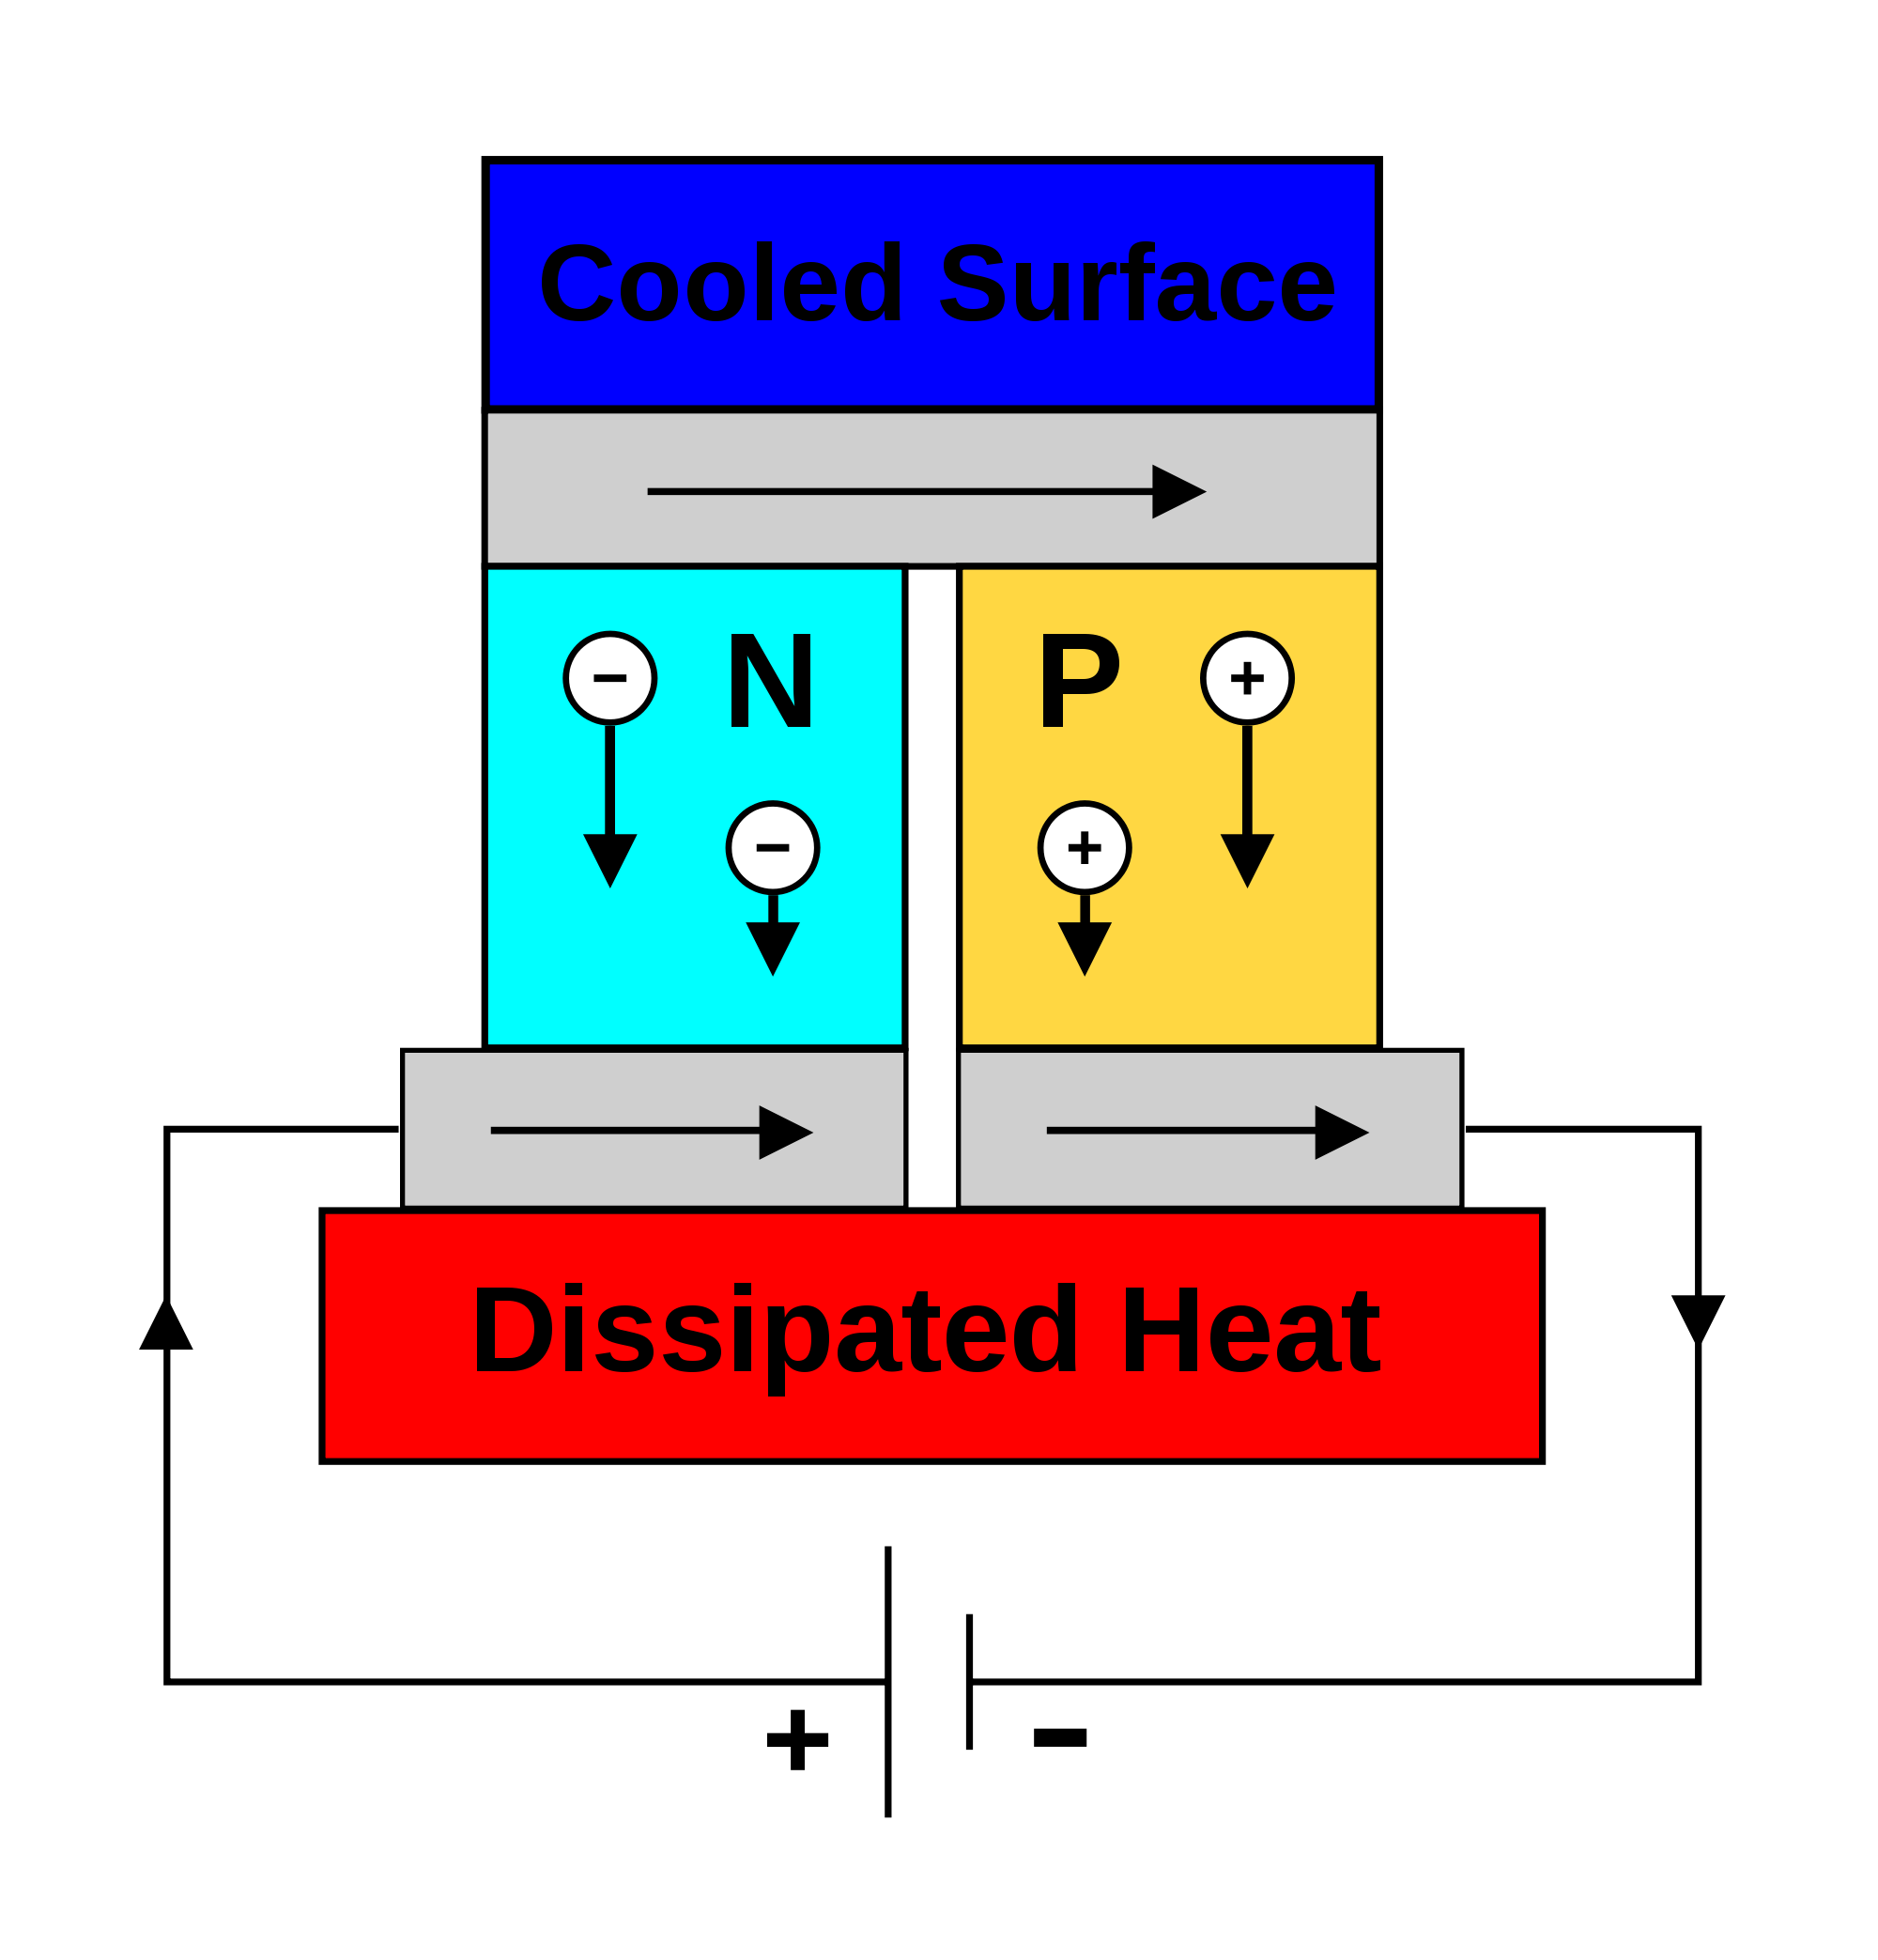
\includegraphics[width=5cm]{images/peltierEffect}
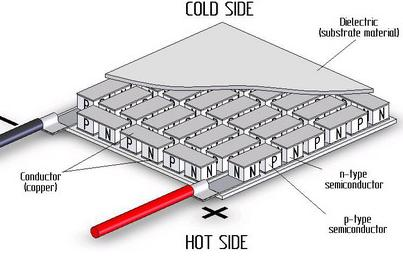
\includegraphics[width=5cm]{images/schematic-diagram-of-peltier-module}
\end{figure}
\end{frame}
}

\subsection{Rendu tactile}
\begin{frame}{Rendu tactile}
\begin{itemize}
\item Contrôle simple la plupart des cas (ex: 1 vibreur)
\begin{figure}
\centering
\includegraphics[width=\linewidth]{images/schema_haptique2}{}
\end{figure}
\item Comment rendre un effet tactile continu dans l'espace avec un nombre limité de vibreurs?
\end{itemize}
\begin{itemize}
\item Exemple : Tactile Brush Algorithm \cite{Israr2011}
\end{itemize}
\begin{figure}
\centering
\includegraphics[width=5cm]{images/immersive-tactile-experiences}
\includegraphics[width=5cm]{images/tactile-brush-algorithm}
%{\cite{Israr2011}}
\end{figure}
\end{frame}

{
\setbeamertemplate{frame footer}{\cite{Israr2011}}
\begin{frame}{Rendu tactile - Tactile Brush Algorithm}
\begin{multicols}{2}
\begin{itemize}
\item Basé sur 2 illusions
\begin{itemize}
\item Apparent tactile motion
\begin{itemize}
\item $SOA = 0.32d + 47.3$
\end{itemize}
\item Phantom tactile sensation
\begin{itemize}
\item $A_1 = \sqrt{1-\beta}.A_v$
\item $A_2 = \sqrt{\beta}.A_v$
\item $\beta = \frac{a}{b}$ 
\end{itemize}
\end{itemize}
\end{itemize}

\begin{figure}
\centering
\includegraphics[width=5cm]{images/tactile-illusions}
\end{figure}
\end{multicols}
\end{frame}

\begin{frame}{Rendu tactile - Tactile Brush Algorithm}
\begin{figure}
\centering
\includegraphics[width=\linewidth]{images/tactile_brush}
\end{figure}
\end{frame}
}

%{
%\setbeamertemplate{frame footer}{\copyright Immersion}
%\subsection{Demo}
%\begin{frame}{Demo}
%\begin{itemize}
%\item Terminal android avec vibreur
%\item SDK Immersion
%\item Exemples d'applications (PlayStore)
%\begin{itemize}
%\item Haptic Effect Preview
%\item Content Portal
%\end{itemize}
%\end{itemize}
%
%\begin{figure}
%\centering
%\includegraphics[width=2cm]{images/hapticpreview}
%\includegraphics[width=2cm]{images/tactileshowcase}
%\end{figure}
%
%\end{frame}
%}